\documentclass[twoside,11pt]{article}

\usepackage{jmlr2e}
\usepackage{lastpage}
\usepackage{natbib}
\usepackage{enumitem}

%%%%%%%%%%%%%%%%%%%%%%%%%%%%%%%%%%%%%%%%
%% Other packages
%%%%%%%%%%%%%%%%%%%%%%%%%%%%%%%%%%%%%%%%
\usepackage{booktabs}
\usepackage[detect-mode=true]{siunitx}
\usepackage{wrapfig}
\usepackage{xcolor}
\usepackage{graphicx}
\graphicspath{{./figures/}}
\usepackage{amsmath}
\usepackage{amsfonts}
\usepackage{cleveref}
\usepackage{vector} % local
\usepackage[font=small]{caption}
\usepackage{natbib}
\usepackage{subcaption}
\usepackage{adjustbox}
\usepackage{longtable}
\usepackage[flushleft]{threeparttable}
\usepackage{multirow}
\usepackage{dsfont} % \mathds{1}
\usepackage{colortbl}
\usepackage[mode=buildnew]{standalone}
% \usepackage[natbib=true]{biblatex}
\usepackage{tabularx}


\newcommand{\algname}{\text{ARIS}}
\newcommand{\algfullname}{\text{Amortized Rare-Event Importance Sampling}}

\sisetup{separate-uncertainty=true,multi-part-units=single,table-align-uncertainty=true, table-format = -3.2(3), detect-weight=true, detect-family=true, detect-all, input-digits = 0123456789\pi}


\definecolor{juliafunccolor}{HTML}{2e51a2}
\definecolor{juliaparenscolor}{HTML}{f2d71c}
\definecolor{pastelRed}{RGB}{245, 97, 92}
\definecolor{pastelBlue}{RGB}{0, 114, 178}
\definecolor{pastelGreen}{RGB}{0, 158, 115}
\definecolor{pastelPurple}{RGB}{135, 112, 254}
\definecolor{pastelYellow}{RGB}{255, 205, 117}


\definecolor{newcolor}{HTML}{000000}
\newcommand{\new}[1]{{\color{newcolor}#1}}

\newcommand\blfootnote[1]{%
  \begingroup
  \renewcommand\thefootnote{}\footnote{#1}%
  \addtocounter{footnote}{-1}%
  \endgroup
}

%%%%%%%%%%%%%%%%%%%%%%%%%%%%%%%%%%%%%%%%
% Algorithms
%%%%%%%%%%%%%%%%%%%%%%%%%%%%%%%%%%%%%%%%
\usepackage{algorithmicx}
\usepackage{algorithm}
\usepackage{algpseudocode}


%%%%%%%%%%%%%%%%%%%%%%%%%%%%%%%%%%%%%%%%
%% TiKZ and PGF plots
%%%%%%%%%%%%%%%%%%%%%%%%%%%%%%%%%%%%%%%%
\usepackage{tikz}
\usepackage{pgfplots}
\pgfplotsset{compat=newest}


\usetikzlibrary{calc}
\usetikzlibrary{shapes.geometric}
\usetikzlibrary{external}
\usetikzlibrary{patterns}
\usetikzlibrary{shapes,arrows,fit}
\usetikzlibrary{positioning}
\usetikzlibrary{arrows.meta, calc, shapes}
\usetikzlibrary{graphs}
\usetikzlibrary{decorations.pathmorphing}
\usetikzlibrary{decorations.pathreplacing}
\usetikzlibrary{backgrounds}
\usetikzlibrary{shadows}
\usepgfplotslibrary{fillbetween}

\definecolor{blues1}{RGB}{198, 219, 239}
\definecolor{blues2}{RGB}{158, 202, 225}
\definecolor{blues3}{RGB}{107, 174, 214}
\definecolor{blues4}{RGB}{49, 130, 189}
\definecolor{blues5}{RGB}{8, 81, 156}

\definecolor{grays1}{RGB}{219, 219, 219}
\definecolor{grays2}{RGB}{202, 202, 202}
\definecolor{grays3}{RGB}{174, 174, 174}
\definecolor{grays4}{RGB}{130, 130, 130}
\definecolor{grays5}{RGB}{81, 81, 81}

%% For Pendulum
\usetikzlibrary{calc,tikzmark,positioning,shadows,arrows}

\definecolor{pastelred}{RGB}{245,97,92}
\definecolor{steelblue}{rgb}{0.27,0.51,0.71}

% Format Helpers
\newcommand{\ph}[1]{{\textbf{#1}:}} %
\newcommand{\red}[1]{\textcolor{red}{#1}}

%% Math Helpers
\newcommand{\ones}{\mathbf 1}
\newcommand{\reals}{{\mbox{\bf R}}}
\newcommand{\integers}{{\mbox{\bf Z}}}
\newcommand{\symm}{{\mbox{\bf S}}}  % symmetric matrices

\newcommand{\nullspace}{{\mathcal N}}
\newcommand{\range}{{\mathcal R}}
\newcommand{\Rank}{\mathop{\bf Rank}}
\newcommand{\Tr}{\mathop{\bf Tr}}
\newcommand{\diag}{\mathop{\bf diag}}
\newcommand{\card}{\mathop{\bf card}}
\newcommand{\rank}{\mathop{\bf rank}}
\newcommand{\conv}{\mathop{\bf conv}}
\newcommand{\prox}{\mathbf{prox}}

\newcommand{\Expect}{\mathop{\mathbb{E}}}
\newcommand{\Reals}{\mathop{\mathbb{R}}}
\newcommand{\Prob}{\mathop{\bf Prob}}
\newcommand{\Co}{{\mathop {\bf Co}}} % convex hull
\newcommand{\dist}{\mathop{\bf dist{}}}
\DeclareMathOperator*{\argmin}{\arg\!\min}
\newcommand{\epi}{\mathop{\bf epi}} % epigraph
\newcommand{\Vol}{\mathop{\bf vol}}
\newcommand{\dom}{\mathop{\bf dom}} % domain
\newcommand{\intr}{\mathop{\bf int}}
\newcommand{\sign}{\mathop{\bf sign}}

\newcommand{\cf}{{\it cf.}}
\newcommand{\eg}{{\it e.g.}}
\newcommand{\ie}{{\it i.e.}}
\newcommand{\etc}{{\it etc.}}

\newcommand{\mbf}[1]{\boldsymbol{#1}}

\newcommand{\bx}{\mathbf{x}}
\newcommand{\by}{\mathbf{y}}
\newcommand{\bz}{\mathbf{z}}

\usetikzlibrary{pgfplots.colorbrewer}
\usepgfplotslibrary{groupplots}
\usepgfplotslibrary{polar}
\usepgfplotslibrary{smithchart}
\usepgfplotslibrary{statistics}
\usepgfplotslibrary{dateplot}
\usepgfplotslibrary{ternary}

\pgfplotsset{
    colormap={pastelPG}{
        color(0cm)=(pastelPurple)   % Start color: blue
        color(0.5cm)=(white) % Neutral color: white
        color(1cm)=(pastelGreen)    % End color: red
    }
}
\graphicspath{{./figures/}}

\newcommand{\dataset}{{\cal D}}
\newcommand{\fracpartial}[2]{\frac{\partial #1}{\partial  #2}}

\jmlrheading{\#}{2026}{1-\pageref{LastPage}}{9/26; Revised M/YY}{M/YY}{21-0000}{Lea M. Hadzic, Harrison Delecki, and Mykel J. Kochenderfer}

\ShortHeadings{Amortized Rare-Event Importance Sampling}{Hadzic, Delecki, and Kochenderfer}

\firstpageno{1}

\RequirePackage{color}

% --------------------------------------------------------------
\begin{document}

\title{Amortized Rare-Event Importance Sampling}

\author{\name Lea M. Hadzic \email lea@cs.stanford.edu \\
       \addr Department of Computer Science \\
       Stanford University\\
       Stanford, CA 94305, USA
       \AND
       \name Harrison Delecki \email hdelecki@alumni.stanford.edu \\
       \addr Department of Aeronautics and Astronautics\\
       Stanford University\\
       Stanford, CA 94305, USA
       \AND
       \name Mykel J. Kochenderfer \email mykel@stanford.edu \\
       \addr Department of Aeronautics and Astronautics\\
       Stanford University\\
       Stanford, CA 94305, USA
       }

\editor{My editor}

\maketitle

% ==============================================================
% 0. ABSTRACT
% ==============================================================
\begin{abstract}%
Estimating the probability of rare events is a fundamental challenge in probabilistic modeling with critical applications in safety validation, risk assessment, and reliability analysis. Standard Monte Carlo methods become prohibitively expensive when event probabilities are extremely small, often requiring billions of samples for acceptable accuracy. While adaptive importance sampling methods can improve efficiency by iteratively refining proposal distributions, standard approaches typically fit a separate proposal for each failure threshold. We introduce \algfullname{} (\algname{}), which amortizes proposal learning by fitting one shared model and reusing it across failure thresholds instead of refitting for each one. By jointly modeling system inputs and robustness values, \algname{} obtains threshold-specific proposals by truncating the learned robustness distribution. We demonstrate the approach on benchmark problems spanning unimodal, multimodal-tail, and isotropic failure geometries, together with a 150-dimensional closed-loop driving setting. In the driving setting, a single adaptive run achieves curve-estimation error comparable to oracle-tuned adaptive multilevel splitting with substantially fewer simulator evaluations, while substantially outperforming independently refitted proposals. The results also identify regimes in which the advantage diminishes, particularly when relevant failure structure is difficult to discover or estimate reliably.
\end{abstract}

% Five keywords.
\begin{keywords}
rare-event estimation, adaptive importance sampling, proposal learning, robustness-conditioned generative modeling, safety validation
\end{keywords}

% ==== START MAIN TEXT ====

% ==============================================================
% 1. INTRODUCTION
% ==============================================================
\section{Introduction}

% Problem setup.
Estimating the probability of rare events is a central problem in probabilistic modeling, with applications to risk management, reliability analysis, and safety validation \citep{corso2020survey, melchers2018structural, komljenovic2016assetrisk}. In these settings, the events of interest, such as a safety violation, occur with extremely low probability under normal operating conditions but carry severe consequences such as loss of life. Accurate estimation of these probabilities is essential for quantifying risk and supporting high-stakes decisions. We assume access to a simulator with random input $X \sim p(\cdot)$, where $p$ is the nominal distribution over possible inputs. The simulator maps a realization $x$ to a system trajectory, and failures are defined through a robustness function $\rho : \mathcal{X} \to \mathbb{R}$ that assigns a scalar safety score to the resulting system behavior. An input $x$ is considered a failure if $\rho(x) \leq \gamma$, for some threshold $\gamma$. The goal is to efficiently estimate the failure probability
\begin{equation*}
    P_{\text{fail}} = P(\rho(X) \leq \gamma).
\end{equation*}
This formalization captures a broad class of rare-event problems, including safety violations in dynamical systems and constraint violations in optimization under uncertainty. The robustness-function formalism follows signal temporal logic semantics \citep{fainekos2009robustness, donze2010robust}.

% Why this is hard.
Standard Monte Carlo methods are often infeasible in the rare-event setting because the number of required samples grows inversely with the probability of the event. For probabilities on the order of $10^{-9}$, this can require upwards of $10^{11}$ samples to achieve acceptable accuracy \citep{owen2013monte}. The challenge becomes more severe in high-dimensional settings, where the input $x$ may encode a long-horizon disturbance sequence for a dynamic system operating under uncertainty. In such cases, the failure region often occupies a vanishingly small, irregular subset of the input space. These regions are frequently multimodal and defined implicitly through complex forward simulations. As dimensionality increases, standard sampling methods become increasingly inefficient due to the curse of dimensionality and the low probability mass near the failure boundary.

% Existing solution and its limitation. 
Importance sampling (IS) provides a principled way to address this challenge by drawing samples from a proposal distribution that concentrates on failure-prone regions \citep{owen2013monte,rubinstein2016simulation}. By reweighting these samples appropriately, IS yields unbiased estimates and can substantially reduce variance. However, designing effective proposal distributions is difficult in high dimensions. Standard parametric families often fail to capture the geometry of rare-event regions, and handcrafted heuristics may not generalize. Adaptive importance sampling (AIS) methods---such as the cross-entropy method and population Monte Carlo---iteratively refine the proposal distribution using samples from intermediate distributions \citep{rubinstein2004cross,cappe2004population}. These methods can be effective, but fitting a proposal for each target separately does not exploit structure shared across a family of nested failure thresholds.

% Core idea of this paper.
% (what we model → how we use it → why that matters)
In this paper, we propose an approach to rare-event estimation that exploits the nested structure of failure regions induced by varying robustness thresholds. We model the joint distribution over system inputs and robustness, decomposing it into a marginal distribution over robustness and a conditional distribution over inputs given robustness. During adaptation, we fit this joint model while progressively decreasing the intermediate robustness threshold. For any requested threshold, we obtain an input proposal by truncating the learned robustness marginal and marginalizing over the retained robustness values. A single adaptive run can therefore estimate \(P(\rho(X)\leq\gamma')\) across a range of thresholds without additional simulation.

% Contributions.
Our contributions are as follows:
\begin{enumerate}
\vspace{-1mm}
    \item A formulation of adaptive rare-event estimation using a joint model over system inputs and robustness, together with convergence results for the smoothed target and an unbiased proposal-of-origin estimator.
    \item An algorithm that learns a robustness-conditioned proposal while amortizing proposal learning across thresholds, allowing a full failure-probability curve to be estimated from a single adaptive run.
    \item Empirical results showing the finite-budget benefit of sharing proposal learning across thresholds and characterizing when robustness conditioning, failure discovery, and estimator-weight concentration limit performance.
\end{enumerate}

% Roadmap.
The remainder of the paper is organized as follows. \Cref{sec:related} reviews related work on rare-event estimation and adaptive sampling. \Cref{sec:background} formalizes the estimation problem and reviews background on importance sampling. \Cref{sec:method} introduces our method. \Cref{sec:experiments} presents experiments, and \cref{sec:conclusion} concludes with a discussion of limitations and future work.

% ==============================================================
% 2. RELATED WORK
% ==============================================================
\section{Related Work}
\label{sec:related}

% Scope of related work.
Estimating rare-event probabilities is a fundamental problem spanning statistics, engineering, and computational science, with applications ranging from financial risk assessment \citep{komljenovic2016assetrisk}, safety validation of autonomous systems \citep{corso2020survey}, and climate modeling \citep{dessai2004doesclimate}. We review several methods, including nonparametric splitting and sequential Monte Carlo methods, parametric adaptive importance sampling methods, and approaches based on flexible density models. These methods address the challenge that standard Monte Carlo becomes prohibitively expensive when event probabilities are extremely small.

% Nonparametric / splitting methods.
\paragraph{Nonparametric methods.}
Nonparametric approaches avoid the limitations of fixed parametric families by representing the proposal distribution through the samples themselves. Subset simulation \citep{au2001estimation} expresses a rare-event probability as a product of larger conditional probabilities across a sequence of nested failure levels, estimated with MCMC at each level. Adaptive multilevel splitting (AMS) \citep{cerou2007adaptive} and its variants employ similar level-based decompositions but use different resampling and splitting strategies. More generally, sequential Monte Carlo (SMC) samplers \citep{del2006sequential,cerou2012sequential} provide a flexible framework for sampling from sequences of distributions, with applications to rare-event estimation through annealing schedules \citep{neal2001annealed}. Our method similarly constructs a sequence of increasingly rare target levels by progressively decreasing the robustness threshold.

% How our method differs from SMC/splitting.
Many nonparametric methods propagate particles through a sequence of intermediate targets, but do not generally learn an explicit functional model of the proposal as a function of the level parameter. Our conditional model instead fits one robustness-conditioned representation across the adaptive path, with samples contributing at their observed robustness values and threshold-specific proposals obtained by truncation. Despite their flexibility, nonparametric methods can face scalability challenges in high-dimensional spaces, especially when effective transition kernels are difficult to construct \citep{sinha2020neural}. Their performance can also depend on kernel and level-selection choices.

% Parametric adaptive importance sampling.
\paragraph{Adaptive Importance Sampling.}
Parametric AIS methods address the proposal design challenge by iteratively refining proposal distributions within predetermined parametric families. The cross-entropy method (CEM) is a widely used approach in this category, iteratively updating a parametric proposal toward the zero-variance importance distribution \citep{rubinstein2004cross, deboer2005tutorial}. Gaussian mixtures can improve the ability of parametric importance-sampling methods to represent multimodal failure regions \citep{kurtz2013cross}. Improved cross-entropy methods (iCE) further replace the hard elite indicator with a smooth transition across intermediate levels to make greater use of intermediate samples \citep{papaioannou2019improved}. This smoothing serves a different role from the observation model used here: iCE smooths the cross-entropy adaptation objective, whereas we introduce a continuous robustness coordinate to define and fit a joint model over inputs and robustness.

Population Monte Carlo (PMC) \citep{cappe2004population} and adaptive multiple importance sampling (AMIS) \citep{cornuet2012adaptive,marin2014consistency} reuse samples generated by sequences of adaptive proposals. Recycling samples under adaptively chosen proposals requires care when establishing consistency or unbiasedness, which motivates the estimator distinctions made in \cref{sec:estimator}. Defensive importance sampling similarly mixes an adaptive proposal with a broader reference distribution to limit the consequences of proposal misspecification \citep{hesterberg1995weighted,owen2000safe}. We use the same safeguard in the defensive mixture also described in \cref{sec:estimator}.

While parametric AIS methods are computationally efficient and easy to implement, their performance depends on how well the chosen family represents the relevant failure geometry. This can be difficult in high-dimensional or multimodal problems.

% Flexible density models
\paragraph{Flexible density modeling approaches.}
Recent advances have expanded the toolkit for rare-event estimation beyond traditional parametric and nonparametric methods by leveraging flexible density modeling techniques. These approaches recognize that the key bottleneck is often the limited expressiveness of proposal distributions rather than the underlying algorithmic framework. Normalizing flows \citep{papamakarios2021normalizing} have emerged as useful models for sampling and rare-event estimation. These models transform simple base distributions into complex target distributions through sequences of invertible transformations. Applications include modeling failure distributions directly \citep{sinha2020neural,gao2023rareflows,ye2024flow} and incorporating flows within MCMC schemes for improved mixing \citep{sinha2020neural}. Diffusion models have also been used to generate diverse failure scenarios in safety validation \citep{delecki2024diffusion}. The formulation developed here is not tied to a particular conditional density estimator and can be instantiated with Gaussian mixtures or more flexible conditional models.

% Positioning our contribution.
Our work builds on the insight that rare-event estimation can benefit from explicitly modeling the joint distribution over system inputs and their associated robustness or safety scores. This perspective leverages the nested structure of failure regions: more restrictive failure criteria define subsets of less restrictive failure regions. By conditioning a density model on robustness, we represent variation across these levels within a single fitted model and obtain threshold-specific proposals by truncation. We use the term \emph{amortized} in this sense of sharing proposal learning across failure thresholds, rather than in the amortized-inference sense of learning an inference map across datasets or observations \citep{kingma2014auto}.

% Closest comparison: splitting.
The closest comparison is to splitting methods. Subset simulation and AMS estimate rare-event probabilities through a sequence of nested levels, while our method learns an explicit robustness-conditioned proposal across the adaptive path. Both exploit structure shared across failure levels, but in different forms: splitting propagates a particle population from level to level, whereas our approach retains a fitted conditional model that can be queried at multiple thresholds. We compare against splitting empirically in \cref{sec:experiments}. The relative advantage depends on the failure geometry, discovery behavior, and finite simulation budget.

% ==============================================================
% 3. PRELIMINARIES
% ==============================================================
\section{Preliminaries}
\label{sec:background}

In this section, we provide necessary background on failure probability estimation, importance sampling, and adaptive importance sampling.

Let $X \in \mathcal{X}$ denote the random input to the system under test, with nominal density $p(x)$. In trajectory-based applications, a realization $x$ of $X$ may represent a sequence of disturbances that induces a system trajectory through the simulator. The robustness function $\rho:\mathcal{X}\to\mathbb{R}$ assigns a scalar outcome to each input and failure occurs when $\rho(x)\leq\gamma$.

% Failure distribution.
The density of inputs conditioned on failure is
\begin{equation}
    \label{eq:failure-distribution}
    p(x \mid \rho(x) \leq \gamma)
    =
    \frac{
        p(x) \mathds{1}\{\rho(x) \leq \gamma\}
    }{
        \int p(x') \mathds{1}\{\rho(x') \leq \gamma\} dx'
    }
\end{equation}
where $\mathds{1}\{\cdot\}$ is the indicator function. The denominator is the total probability of failure, which we denote by $P_{\text{fail}}$. For high-dimensional inputs and black-box system models, this integral is generally unavailable in closed form, so we estimate it from system evaluations.

% Section 3.1
% --------------------------------------------------------------
\subsection{Failure Probability Estimation}

% Define failure probability.
Failure probability estimation is the problem of estimating the denominator of \cref{eq:failure-distribution}, or the expected value
\begin{equation*}
    P_{\text{fail}}
=
\mathbb{E}_{X\sim p}
\left[
    \mathds{1}\{\rho(X)\leq\gamma\}
\right].
\end{equation*}
Monte Carlo (MC) estimates $P_{\text{fail}}$ using $N$ independent inputs $x_i \sim p$ as
\begin{equation*}
    \hat{P}^{\text{MC}}_{\text{fail}}
    =
    \frac{1}{N}
    \sum_{i=1}^N
    \mathds{1}\{\rho(x_i)\leq\gamma\}.
\end{equation*}

% Why Monte Carlo is expensive.
It can be shown that for a desired level of relative accuracy $\epsilon_{\text{rel}}$ on the estimated probability, the required number of samples is
\begin{equation*}
    N > \frac{(1 - P_{\text{fail}})}{ P_{\text{fail}} \epsilon^2_{\text{rel}}}.
\end{equation*}
In safety-critical settings, $P_{\text{fail}}$ may be very small, for example $10^{-9}$. This case would require roughly $10^{11}$ samples to achieve a relative error under $10\%$, which is impractical for many applications \citep{owen2013monte}.

% Section 3.2
% --------------------------------------------------------------
\subsection{Importance Sampling}

% What importance sampling does.
Importance sampling (IS) can reduce estimator variance by sampling more frequently from failure-prone regions of the input space. Given inputs $x_i$ sampled from a proposal distribution $q$, the IS estimate is
\begin{equation}
    \label{eq:is-estimate}
    \hat{P}^\text{IS}_{\text{fail}}
    =
    \frac{1}{N}
    \sum_{i=1}^N
    w(x_i)
    \mathds{1}\{\rho(x_i)\leq\gamma\}
\end{equation}
where the samples are weighted according to their importance weight
\begin{equation*}
    w(x) = p(x)/q(x).
\end{equation*}
The IS estimator is unbiased if $q(x)>0$ whenever $p(x)\mathds{1}\{\rho(x)\leq\gamma\}>0$. The zero-variance importance sampling distribution $q^*(x)$ is the failure distribution itself:
\begin{equation*}
    q^*(x)=\frac{p(x)\mathds{1}\{\rho(x)\leq\gamma\}}{P_{\text{fail}}}.
\end{equation*}
Thus, the zero-variance proposal is the nominal input distribution conditioned on failure. It is unavailable in practice because its normalization constant is $P_{\text{fail}}$, the quantity being estimated.

% The actual difficulty.
The key challenge is constructing a proposal that covers the failure-inducing region of the input space. Poor coverage can produce high-variance estimates, particularly when the input dimension is large.

% Section 3.3
% --------------------------------------------------------------
\subsection{Adaptive Importance Sampling}

% Adaptive importance sampling / CEM.
Adaptive importance sampling (AIS) methods iteratively adapt a proposal toward the optimal IS distribution \citep{bugallo2017adaptive}. Some AIS methods propagate and reweight a population of samples to approximate a sequence of target distributions \citep{cappe2004population, martino2017layered, elvira2017improving}. Such methods can become costly as the input dimension increases. Other AIS approaches iteratively fit a parametric input proposal $q_{\theta}(x)$ \citep{rubinstein2004cross, cornuet2012adaptive}.

We focus on an adaptive procedure inspired by the cross-entropy method (CEM) \citep{rubinstein2004cross}. At iteration $k$, CEM updates the parametric proposal by minimizing the Kullback--Leibler (KL) divergence from the optimal IS proposal
\begin{equation*}
    \theta^{(k+1)}
    =
    \argmin_{\theta}
    D_{\mathrm{KL}}
    \left(
        q^*
        \,\|\,
        q_{\theta}
    \right).
\end{equation*}

Due to the rarity of failures, there may be too few samples from the target failure region to estimate this objective reliably. CEM therefore introduces an intermediate threshold $\gamma^{(k)}$. Given inputs $x_i\sim q_{\theta^{(k)}}$, the next threshold is chosen from the lower $\alpha$-quantile of the sampled robustness values subject to the final failure threshold $\gamma_{\text{fail}}$,
\begin{equation*}
    \gamma^{(k+1)}
    =
    \max
    \left(
        \gamma_{\text{fail}},
        \rho_{\alpha}^{(k)}
    \right)
\end{equation*}
where $\rho_{\alpha}^{(k)}$ is the $\alpha$-quantile of $\{\rho(x_i)\}_{i=1}^N$. The proposal update then uses inputs satisfying the new intermediate threshold
\begin{equation}
\label{eq:cem-sample-obj}
    \theta^{(k+1)}
    \approx
    \argmin_{\theta}
    -\frac{1}{N}
    \sum_{i=1}^N
    \mathds{1}\{\rho(x_i)\leq\gamma^{(k+1)}\}
    w(x_i)
    \log q_{\theta}(x_i).
\end{equation}
The CEM update at iteration $k$ can be summarized as
\begin{enumerate}
    \item Sample inputs $\{x_i\}_{i=1}^N$ from $q_{\theta^{(k)}}$.
    \item Evaluate $\rho(x_i)$ for each input.
    \item Compute $\rho_{\alpha}^{(k)}$, the $\alpha$-quantile of $\{\rho(x_i)\}_{i=1}^N$.
    \item Set $\gamma^{(k+1)} = \max(\gamma_{\text{fail}}, \rho_{\alpha}^{(k)})$.
    \item Update $q_{\theta}$ using \cref{eq:cem-sample-obj}.
\end{enumerate}

Standard CEM adapts a proposal toward a single target failure threshold through a sequence of intermediate levels. To estimate probabilities at multiple target thresholds, the procedure is typically run separately for each target. Our method instead learns how the input distribution varies with robustness, allowing proposal learning to be shared across thresholds.

% ==============================================================
% 4. METHODS
% ==============================================================
\section{Methods}
\label{sec:method}

We present \algfullname{} (\algname{}), an approach to rare-event estimation based on a joint model of inputs and robustness values. We first define the joint proposal, then describe its optimization and implementation.

% Section 4.1
% --------------------------------------------------------------
\subsection{Joint Distribution for Rare Event Estimation}

% Nested failure regions.
Failure sets are nested across robustness thresholds. For $\gamma_1<\gamma_2$,
\[
    \{x:\rho(x)\leq\gamma_1\}
    \subseteq
    \{x:\rho(x)\leq\gamma_2\}.
\]
The corresponding conditional input distributions satisfy
\begin{align*}
    p(x \mid \rho(x)\leq\gamma_1)
    &=
    \frac{
        p(x \mid \rho(x)\leq\gamma_2)
        \mathds{1}\{\rho(x)\leq\gamma_1\}
    }{
        \int
        p(x' \mid \rho(x')\leq\gamma_2)
        \mathds{1}\{\rho(x')\leq\gamma_1\}
        dx'
    } \\
    &=
    \frac{
        p(x \mid \rho(x)\leq\gamma_2)
        \mathds{1}\{\rho(x)\leq\gamma_1\}
    }{
        P(\rho(X)\leq\gamma_1
        \mid
        \rho(X)\leq\gamma_2)
    }.
\end{align*}
The denominator is the probability of satisfying the stricter threshold $\gamma_1$ conditional on satisfying $\gamma_2$. A proof is given in \cref{app:failure-nesting}.

% The joint-model idea.
Rather than fitting a separate sublevel distribution $p(x\mid\rho(x)\leq\gamma)$ at each threshold, we model how the input distribution varies with the robustness value itself. Let $R=\rho(X)$. Formally, the joint distribution of $(X,R)$ decomposes into the robustness marginal and the conditional distribution of inputs at each robustness level. This level-set conditioning is the object we model. Sublevel distributions are obtained by integrating over robustness. 

The sublevel conditional at threshold $\gamma$ is obtained by integrating the level-set conditionals
\begin{equation}
    \label{eq:exact-joint-integral}
    p(x\mid R\leq\gamma)
    \propto
    \int_{-\infty}^{\gamma}
    p(x\mid R=r)\,dP_R(r).
\end{equation}

Modeling the level-set conditional $p(x\mid R=r)$ preserves the dependence of the input distribution on robustness. The sublevel family then follows by integration for every threshold. Modeling only $p(x\mid R\leq\gamma)$ would instead combine all robustness levels below $\gamma$ into a single conditional and would require a separate model, or additional structure, to recover the level-set dependence.

A single model of the robustness-indexed conditional family can therefore define proposals across all thresholds. The next section introduces a continuous observation model that makes this joint representation suitable for density estimation.

% Section 4.2
% --------------------------------------------------------------
\subsection{A Smoothed Robustness Observation Model}
\label{sec:sigma-model}

Because $R=\rho(X)$ is deterministic given $X$, the joint distribution of $(X,R)$ is supported on the graph $\{(x,\rho(x))\}$ and is singular with respect to Lebesgue measure on $\mathcal{X}\times\mathbb{R}$. This makes direct fitting with an absolutely continuous joint density ill-posed. We therefore introduce a continuous robustness observation model. For $\sigma>0$, let
\[
    \tilde{R}
    =
    \rho(X)+\varepsilon,
    \qquad
    \varepsilon\sim\mathcal{N}(0,\sigma^2),
\]
which induces the joint density
\begin{equation}
    \label{eq:sigma-joint}
    \tilde{p}_\sigma(x,r)
    =
    p(x)\,k_\sigma(r-\rho(x))
\end{equation}
where $k_\sigma$ is the Gaussian density with mean zero and standard deviation $\sigma$. Integrating over $r$ recovers the nominal input density $p(x)$ for every $\sigma>0$, so smoothing changes the proposal-learning target but not the nominal distribution being estimated.

Integrating \cref{eq:sigma-joint} over $r\leq\gamma$ gives
\begin{equation}
    \label{eq:probit-lemma}
    \int_{-\infty}^{\gamma}
    \tilde{p}_\sigma(x,r)\,dr
    =
    p(x)\,
    \Phi\!\left(
        \frac{\gamma-\rho(x)}{\sigma}
    \right)
\end{equation}
where $\Phi$ is the standard normal cumulative distribution function. The factor
\[
    \Phi\!\left(
        \frac{\gamma-\rho(x)}{\sigma}
    \right)
\]
is a probit relaxation of $\mathds{1}\{\rho(x)\leq\gamma\}$ and converges pointwise to the hard indicator for $\rho(x)\neq\gamma$ as $\sigma\to0$.

Three properties follow; proofs are given in \cref{app:theory}.
\begin{enumerate}
    \item \textbf{Well-posedness.}
    For every $\sigma>0$, $\tilde{p}_\sigma$ is an absolutely continuous joint density. The corresponding density-fitting objective is therefore well-defined for proposal families with adequate support.

    \item \textbf{Convergence.}
    Under mild regularity conditions, the smoothed sublevel target converges in total variation to the exact conditional distribution as $\sigma\to0$. For small $\sigma$, the approximation error decreases roughly linearly with $\sigma$ and depends on how much probability mass lies near the threshold (\cref{prop:smoothing-convergence}).

    \item \textbf{Estimator validity.}
    The final importance-sampling estimator uses the proposal's marginal density over $x$ (\cref{sec:proposal-optimization}). The smoothing parameter $\sigma$ affects proposal learning but does not appear in the estimator itself.
\end{enumerate}

\paragraph{Choosing $\sigma$.}
The convergence result motivates decreasing $\sigma$ as the smoothed target approaches the hard-indicator limit, but it does not by itself prescribe an adaptive schedule for a fitted proposal. We therefore treat $\sigma$ as a proposal-learning parameter rather than part of the estimator.

\paragraph{Scope of the rate.}
Property 2 applies to the smoothed target family, not directly to the fitted proposal. It assumes that the conditional model represents the smoothed target exactly. Approximation error from a misspecified proposal family is separate. In particular, smoothing cannot compensate for a proposal family that fails to cover the relevant failure geometry. The safeguards in \cref{sec:estimator} preserve estimator validity under imperfect proposals but do not remove this approximation error.

For $\sigma>0$, we approximate the smoothed joint density with
\begin{equation*}
    q_{\theta,\psi}(x,r)
    =
    q_{\psi}(r)\,q_{\theta}(x\mid r)
\end{equation*}
where $q_{\psi}$ models the robustness marginal and $q_{\theta}$ models the conditional input distribution at robustness value $r$.

For a given threshold $\gamma$, truncating the learned robustness marginal induces the input proposal
\begin{equation*}
    q_X^\gamma(x)
    =
    \int_{-\infty}^{\gamma}
    q_{\psi}(r\mid r\leq\gamma)\,
    q_{\theta}(x\mid r)\,dr.
\end{equation*}
Only a one-dimensional truncation of $q_{\psi}$ is required to construct the proposal at a new threshold without needing additional system simulation or proposal refitting. Because all threshold-specific proposals are obtained from the same fitted joint model, they share a common robustness-conditioned representation. This is how the proposed method shares proposal learning across thresholds: samples collected at one robustness level contribute to the same conditional model used to construct proposals at other levels.

To sample from $q_X^\gamma$, we first draw $r\sim q_{\psi}(\cdot\mid r\leq\gamma)$ and then draw $x\sim q_{\theta}(\cdot\mid r)$. The smoothed formulation above provides a continuous proposal-learning target for $\sigma>0$.

\paragraph{Use in the main method.}
Observation smoothing is optional. The main experiments use the observed robustness value $r=\rho(x)$ when fitting the joint model, corresponding to $\sigma=0$. Accordingly, \cref{sec:proposal-optimization} describes the fitting objective used by the main method. At \(\sigma=0\), the joint distribution of \((X,R)\) is singular, so direct density fitting is well posed only after restricting the proposal family. In practice, we bound mixture-component covariances away from singularity: the full-covariance family uses an additive covariance ridge when its determinant falls below a numerical threshold, while the structured family floors its diagonal covariance component. The implementation also adds a small numerical jitter with standard deviation \(10^{-4}\) to the robustness coordinate during conditional-model fitting to avoid singular covariance estimates from the near-deterministic relation \(r=\rho(x)\).

These restrictions stabilize the finite-sample density fit but do not make the fitted joint distribution converge to the singular population target. The estimator depends on the fitted model only through the induced input marginal $q_X^\gamma$. Because the regularized conditional densities have full support, $q_X^\gamma$ satisfies the support condition required for importance sampling. Approximation error in the joint model therefore affects estimator efficiency rather than the target probability being estimated.

When smoothing is enabled, the fitting procedure additionally reweights observations using the probit factor implied by \cref{eq:probit-lemma} and jitters the robustness value supplied to the conditional model. The sampling and probability-estimation rules are unchanged.

% Section 4.3
% --------------------------------------------------------------
\subsection{Optimizing the Proposal}
\label{sec:proposal-optimization}

% Objective.
The joint model is shared across robustness thresholds, so we fit it using all input--robustness pairs collected during adaptation rather than fitting a separate model at each intermediate threshold. Let
\[
    q_{\theta,\psi}(x,r)
    =
    q_{\psi}(r)\,
    q_{\theta}(x\mid r).
\]
The fitting objective is the expected negative log likelihood of the joint model under the nominal input distribution
\begin{equation}
    \label{eq:joint-fit-objective}
    \mathcal{L}(\theta,\psi)
    =
    -
    \mathbb{E}_{X\sim p}
    \left[
        \log q_{\theta,\psi}(X,\rho(X))
    \right].
\end{equation}
This objective learns the relationship between inputs and robustness values across the range represented in the collected data. Intermediate thresholds affect where new samples are collected, but do not directly restrict which previous samples are used to fit the joint model.

% Using importance sampling to fit the joint model.
\paragraph{Proposal fitting.}
Samples are collected from a sequence of adaptive input proposals rather than directly from $p(x)$. For a sample $x$ drawn from proposal $q_X'(x)$, define the proposal-fitting weight
\begin{equation}
    \label{eq:fit-weight}
    w_{\mathrm{fit}}(x)
    =
    \frac{p(x)}{q_X'(x)}.
\end{equation}
Importance weighting then gives
\begin{equation}
    \label{eq:weighted-joint-fit}
    \mathcal{L}(\theta,\psi)
    =
    -
    \mathbb{E}_{X\sim q_X'}
    \left[
        w_{\mathrm{fit}}(X)
        \log q_{\theta,\psi}(X,\rho(X))
    \right].
\end{equation}
Implementation details for the fitting weights are given in \cref{app:reproducibility}.

% Fitting weights vs. estimation weights.
\paragraph{Fitting weights vs.\ estimation weights.}
The weights above are used only to fit the joint proposal. The final failure-probability estimator instead uses the marginal density of the sampled input. Under the two-stage sampler, $r \sim q_\psi(\cdot \mid r \leq \gamma)$ followed by $x \sim q_\theta(\cdot \mid r)$, the induced input density is
\begin{equation*}
    q_X^\gamma(x)
    =
    \int_{-\infty}^{\gamma}
    q_\psi(r \mid r \leq \gamma)\,
    q_\theta(x \mid r)\,dr.
\end{equation*}
Because the failure event depends only on $x$, the corresponding estimation weight is
\begin{equation*}
    w_{\mathrm{est}}(x)
    =
    \frac{p(x)}{q_X^\gamma(x)}
\end{equation*}
where the one-dimensional integral defining $q_X^\gamma$ is evaluated by quadrature. Evaluating the joint density at the realized robustness value, $q_\psi(\rho(x))q_\theta(x\mid\rho(x))$, does not equal the density from which $x$ was sampled and therefore does not produce a valid importance-sampling weight. Marginalizing over the auxiliary robustness variable also Rao--Blackwellizes the weight relative to conditioning on a particular sampled value of $r$.

% Unbiasedness.
\paragraph{Unbiasedness.}
Fix the evaluation threshold $\gamma_{\mathrm{fail}}$. For any proposal $q_X(x)$ whose density can be evaluated exactly, and with support wherever $p(x)\mathds{1}\{\rho(x)\leq\gamma_{\mathrm{fail}}\}>0$,
\[
    \mathbb{E}_{X\sim q_X}
    \left[
        \mathds{1}\{\rho(X)\leq\gamma_{\mathrm{fail}}\}
        \frac{p(X)}{q_X(X)}
    \right]
    =
    P_{\mathrm{fail}}.
\]
The smoothing parameter $\sigma$ does not appear in this estimator. In implementations where $q_X$ is evaluated numerically, this exact unbiasedness statement is subject to the corresponding numerical integration error.

The same unbiasedness result holds under adaptive proposal selection when each proposal is fixed conditional on the preceding sampling history. By the tower property, proposal-of-origin batch estimates remain unbiased when any batch weights or inclusion rules are determined independently of the current batch outcomes. We prove this result in \cref{app:adaptive-unbiasedness} and define the corresponding estimator in \cref{sec:alg-desc}.

Outcome-dependent selection can introduce bias. For example, discarding batches because they contain no target failures conditions on the quantity being estimated and biases the estimate upward.

This argument applies to proposal-of-origin importance sampling. It does not establish unbiasedness for a pooled balance-MIS estimator whose mixture denominator contains later proposals fitted using earlier samples. We treat that pooled estimator separately in \cref{sec:alg-desc}.

For proposal-of-origin importance sampling, because the nominal density $p(x)$ is known and the proposal marginal $q_X(x)$ is evaluated directly, the estimator uses ordinary importance weights rather than self-normalized weights and is unbiased under the support conditions above. Self-normalized importance sampling would generally introduce finite-sample bias. Unbiasedness also does not guarantee low variance. For a fixed failure threshold $\gamma_{\mathrm{fail}}$, finite variance requires
\[
    \int_{\{x:\rho(x)\leq\gamma_{\mathrm{fail}}\}}
    \frac{p(x)^2}{q_X(x)}\,dx
    <
    \infty.
\]
A proposal that assigns too little density to part of the failure region can therefore yield an unbiased but high-variance estimator. The defensive mixture in \cref{sec:estimator} provides a lower bound on the proposal density and corresponding upper bound on the importance weights.

% Factorized loss.
Because $q_{\theta,\psi}(x,r)=q_\psi(r)q_\theta(x\mid r)$, the fitting objective separates as
\begin{align}
    \mathcal{L}(\theta,\psi)
    ={}&
    -
    \mathbb{E}_{X\sim q_X'}
    \left[
        w_{\mathrm{fit}}(X)
        \log q_\psi(\rho(X))
    \right]
    \nonumber\\
    &-
    \mathbb{E}_{X\sim q_X'}
    \left[
        w_{\mathrm{fit}}(X)
        \log q_\theta(X\mid\rho(X))
    \right].
    \label{eq:factorized-fit}
\end{align}
The parameters $\psi$ and $\theta$ can therefore be optimized separately. Given samples $\{x_n\}_{n=1}^N$ from $q_X'$, with $r_n=\rho(x_n)$, the two components are estimated by
\begin{align}
    \mathcal{L}(\psi)
    &\approx
    -\frac{1}{N}
    \sum_{n=1}^N
    w_{\mathrm{fit}}(x_n)
    \log q_\psi(r_n),
    \\
    \mathcal{L}(\theta)
    &\approx
    -\frac{1}{N}
    \sum_{n=1}^N
    w_{\mathrm{fit}}(x_n)
    \log q_\theta(x_n\mid r_n).
    \label{eq:is-loss}
\end{align}

% Adaptive data collection.
\paragraph{Adaptive data collection.}
Although the fitting objective uses all accumulated samples, directly sampling from a proposal truncated at the final failure threshold can be ineffective before the model has observed sufficiently low robustness values. We therefore use a sequence of intermediate thresholds to control where new data are collected.

Let $\gamma^{(k)}$ denote the threshold used to construct the input proposal at iteration $k$. After drawing a batch and evaluating its robustness values, we set
\[
    \gamma^{(k+1)}
    =
    \max\!\left(
        \gamma_{\mathrm{fail}},
        \rho_\alpha^{(k)}
    \right)
\]
where $\rho_\alpha^{(k)}$ is the lower $\alpha$-quantile of the current batch. The next input proposal is obtained by truncating the updated robustness marginal at $\gamma^{(k+1)}$.

The threshold therefore controls the distribution of newly collected samples, not the subset of accumulated samples used for fitting. As adaptation moves toward lower robustness, the shared conditional model receives increasing coverage of the regions needed to construct proposals for more restrictive thresholds while retaining information collected at earlier robustness levels.

% Section 4.4
% --------------------------------------------------------------
\subsection{Algorithm Description and Implementation}
\label{sec:alg-desc}

% Sample reuse.
\paragraph{Sample reuse.}
We reuse samples across iterations both for proposal fitting and, with a separate weighting rule, for probability estimation. Because each batch is drawn from a different adaptive proposal, the fitting and estimation uses must be distinguished.

For proposal-of-origin importance sampling, let $q_X^{(k)}$ denote the marginal input proposal that generated batch $k$. The corresponding batch estimate at evaluation threshold $\gamma$ is
\begin{equation}
    \label{eq:batch-is}
    \hat{P}_k(\gamma)
    =
    \frac{1}{N}
    \sum_{i=1}^{N}
    \mathds{1}\{\rho(x_{k,i})\leq\gamma\}
    \frac{p(x_{k,i})}{q_X^{(k)}(x_{k,i})}.
\end{equation}
Averaging these batch estimates preserves the adaptive-IS unbiasedness result in \cref{sec:proposal-optimization}.

For the amortized estimator, we also use balance-heuristic multiple importance sampling (MIS) \citep{veach1995optimally, elvira2019generalized}. The balance-MIS pool contains the $K$ checkpointed proposals, one from each adaptive iteration. With equal batch sizes, define
\begin{equation}
    \label{eq:balance-mixture}
    \bar{q}_X(x)
    =
    \frac{1}{K}
    \sum_{j=1}^{K}
    q_X^{(j)}(x).
\end{equation}
The corresponding pooled estimate is
\begin{equation}
    \label{eq:balance-mis-estimator}
    \hat{P}_{\mathrm{MIS}}(\gamma)
    =
    \frac{1}{KN}
    \sum_{k=1}^{K}
    \sum_{i=1}^{N}
    \mathds{1}\{\rho(x_{k,i})\leq\gamma\}
    \frac{p(x_{k,i})}{\bar{q}_X(x_{k,i})}.
\end{equation}
The mixture denominator accounts for the density assigned to each sample by all proposals in the pool. Computing \cref{eq:balance-mis-estimator} requires evaluating each checkpointed proposal on the pooled samples, so we retain the samples and proposal parameters from each iteration.

In our adaptive setting, later proposals may have been fitted using earlier samples that also appear in \cref{eq:balance-mis-estimator}. The standard proposal-of-origin tower-property argument therefore does not establish unbiasedness of this pooled estimator. We use balance MIS as the pooled amortized estimator and evaluate its finite-sample behavior empirically. Unless stated otherwise, the amortized methods use \cref{eq:balance-mis-estimator}, while the per-threshold baselines average the proposal-of-origin batch estimates in \cref{eq:batch-is}.

% Reused-sample loss.
Assuming that we draw $N$ samples at each iteration, we estimate the fitting loss at iteration $k$ using all samples collected through that iteration. Let
\[
    w_{\mathrm{fit}}^{(i)}(x)
    =
    \frac{p(x)}{q_X^{(i)}(x)}
\]
denote the proposal-of-origin fitting weight for a sample drawn at iteration $i$, then
\begin{align}
    \label{eq:reused-fit-loss}
    \mathcal{L}^{(k)}(\theta)
    &\approx
    -\frac{1}{kN}
    \sum_{i=1}^k
    \sum_{n=1}^N
    w_{\mathrm{fit}}^{(i)}(x_n^i)\,
    \log q_{\theta}(x_n^i\mid r_n^i)
    \\
    \mathcal{L}^{(k)}(\psi)
    &\approx
    -\frac{1}{kN}
    \sum_{i=1}^k
    \sum_{n=1}^N
    w_{\mathrm{fit}}^{(i)}(x_n^i)\,
    \log q_{\psi}(r_n^i)
    \nonumber
\end{align}
where $r_n^i=\rho(x_n^i)$. In practice, the proposal-fitting weights may be clamped to improve numerical stability in the density fit. This stabilization is applied only during proposal learning. The failure-probability estimator uses the raw marginal importance weights.

% Model family selection.
\paragraph{Model family selection.}
The framework permits different tractable model families for $q_{\psi}$ and $q_{\theta}$. The robustness marginal $q_{\psi}$ can be any univariate density that supports truncation, such as a Gaussian or Gaussian mixture model (GMM). The conditional input model $q_{\theta}$ can be any tractable conditional density model.

For a GMM, we fit a joint model over $(x,r)$ by expectation maximization and obtain $q_{\theta}(x\mid r)$ by conditioning on the robustness value $r$. Alternatively, a conditional normalizing flow can be trained by gradient descent on the fitting loss \citep{papamakarios2021normalizing}. The corresponding gradient estimate is
\begin{equation*}
    \nabla_{\theta}\mathcal{L}(\theta)
    \approx
    -\frac{1}{N}
    \sum_{n=1}^N
    w_{\mathrm{fit}}(x_n)\,
    \nabla_{\theta}
    \log q_{\theta}(x_n\mid r_n).
\end{equation*}

% Structured covariance.
\paragraph{Structured covariance at high input dimension.}
Full-covariance conditional models become expensive as the input dimension increases. We therefore use a low-rank-plus-diagonal covariance GMM, which preserves tractable densities and analytic conditioning while reducing the covariance parameterization from quadratic to approximately linear scaling in the input dimension.

Unregularized maximum-likelihood fits can become numerically unstable when adaptation concentrates samples in a small region of the input space. We therefore floor the diagonal covariance component at $10^{-4}$, which keeps the low-rank-plus-diagonal covariance positive definite, and use the estimator safeguards described in \cref{sec:estimator}. The high-dimensional experiments use this structured proposal family. Exact rank and regularization settings are reported with the experimental configuration.

% Algorithm.
\paragraph{Algorithm description.}
The full procedure is given in \cref{alg:method}. We initialize the first input proposal as $q_X^{(1)}=p$, set the intermediate threshold $\gamma^1=\infty$, and initialize a buffer for the sampled inputs, robustness evaluations, and proposal information needed for estimation.

At iteration $k$, we draw $N$ inputs from the current proposal $q_X^{(k)}$ and evaluate their true robustness values $\rho(x)$. We then update $q_{\psi}$ and $q_{\theta}$ using all samples collected through iteration $k$, weighted by their proposal-of-origin fitting weights. The intermediate threshold does not mask the fitting data. It determines the truncation used to generate the next batch.

The next threshold is set from the lower $\alpha$-quantile of the most recently observed robustness values,
\[
    \gamma^{(k+1)}
    =
    \max\!\left(
        \gamma_{\mathrm{fail}},
        \rho_\alpha^{(k)}
    \right).
\]
For $k\geq 1$, the proposal for the next iteration is obtained by truncating the updated robustness marginal at $\gamma^{(k+1)}$,
\[
    q_X^{(k+1)}(x)
    =
    \int_{-\infty}^{\gamma^{(k+1)}}
    q_{\psi^{(k+1)}}(r\mid r\leq\gamma^{(k+1)})\,
    q_{\theta^{(k+1)}}(x\mid r)\,dr.
\]

The procedure continues for a fixed number of iterations. After adaptation, we estimate $P_{\mathrm{fail}}$ using the stored samples and the marginal importance weights defined in \cref{sec:proposal-optimization}.

\Cref{alg:method} states the method in its generic form, without the defensive mixture. When the defensive mixture of \cref{sec:estimator} is used, the input proposal $q_X^{(k)}$ is replaced by $q_\eta^{(k)}=(1-\eta)q_X^{(k)}+\eta p$ for sampling and for the corresponding importance weights, while proposal fitting and the intermediate-threshold update continue to use samples from the adaptive component only.

% ==== START ALGORITHM ====

\begin{algorithm}[ht!]
\caption{\algfullname{}}
\label{alg:method}
\algtext*{EndProcedure}%
\algtext*{EndFunction}%
\algtext*{EndFor}
\renewcommand{\algorithmicdo}{}
\begin{algorithmic}[1]

\Require nominal input distribution $p(x)$, robustness function $\rho(x)$,
failure threshold $\gamma_{\mathrm{fail}}$, quantile fraction $\alpha$,
samples per iteration $N$, iterations $K$

\Function{\algname{}}{$p, \rho, \gamma_{\mathrm{fail}}, \alpha, N, K$}

    \State $\mathcal{D} \gets \{\}$ \Comment{Initialize sample buffer}
    \State $q_X^{(1)}(x) \gets p(x)$ \Comment{Initialize input proposal}
    \State $\gamma^{1} \gets \infty$

    \For{$k \in 1:K$}

        \State $x_n \sim q_X^{(k)}$ for $n \in 1:N$
        \Comment{Sample inputs}

        \State $r_n \gets \rho(x_n)$ for $n \in 1:N$
        \Comment{Evaluate robustness}

        \State $w_n
        \gets
        p(x_n)/q_X^{(k)}(x_n)$ for $n \in 1:N$
        \Comment{Proposal-of-origin weights}

        \State $\mathcal{D}
        \gets
        \mathcal{D}
        \cup
        \{(x_n,r_n,w_n,k)\}_{n=1}^{N}$

        \State $\rho_{\alpha}^{(k)}
        \gets
        \textsc{quantile}(\{r_n\}_{n=1}^{N},\alpha)$

        \State $\gamma^{(k+1)}
        \gets
        \max(\gamma_{\mathrm{fail}},\rho_{\alpha}^{(k)})$

        \State $\theta^{(k+1)}
        \gets
        \argmin_{\theta}
        \mathcal{L}^{(k)}(\theta)$
        \Comment{Fit using all samples in $\mathcal{D}$}

        \State $\psi^{(k+1)}
        \gets
        \argmin_{\psi}
        \mathcal{L}^{(k)}(\psi)$
        \Comment{\Cref{eq:reused-fit-loss}}

        \State $q_X^{(k+1)}(x)
        \gets
        \int_{-\infty}^{\gamma^{(k+1)}}
        q_{\psi^{(k+1)}}(r \mid r\leq\gamma^{(k+1)})
        q_{\theta^{(k+1)}}(x\mid r)\,dr$

        \State \textsc{Checkpoint}$(q_X^{(k+1)},\gamma^{(k+1)})$

    \EndFor

    \State \Return $\hat{P}_{\mathrm{fail}}
    \gets
    \textsc{ImportanceSamplingEstimate}
    (\mathcal{D},\gamma_{\mathrm{fail}})$

\EndFunction
\end{algorithmic}
\end{algorithm}

% ==== END ALGORITHM ====


% Section 4.5
% --------------------------------------------------------------
\subsection{Estimator Design}
\label{sec:estimator}

% Raw weights in the estimate.
\paragraph{Raw weights in the estimate.} 
The final estimator uses the raw marginal importance weights defined in \cref{sec:proposal-optimization}. Any weight stabilization, clipping, or clamping is applied only to the proposal-fitting objective. Modifying the estimation weights generally introduces bias because the resulting estimator no longer uses the likelihood ratio $p(x)/q_X(x)$. We therefore leave estimation weights unmodified.

% Defensive mixture.
\paragraph{Defensive mixture.}
To guard against proposal under-coverage, we augment the adaptive input proposal with the nominal distribution
\[
    q_\eta(x)
    =
    (1-\eta)q_X(x)
    +
    \eta p(x)
\]
where $\eta\in(0,1]$. Because $q_\eta(x)\geq\eta p(x)$, the corresponding importance weights satisfy
\[
    w_\eta(x)
    =
    \frac{p(x)}{q_\eta(x)}
    \leq
    \frac{1}{\eta}.
\]
For $M$ independent samples from $q_\eta$, this gives
\[
    \mathrm{Var}(\hat{P}_\eta)
    \leq
    \frac{1}{M}
    \left(
        \frac{P_{\mathrm{fail}}}{\eta}
        -
        P_{\mathrm{fail}}^2
    \right)
    \leq
    \frac{P_{\mathrm{fail}}}{\eta M}.
\]
The defensive mixture therefore bounds the importance weights and the estimator variance even when the adaptive proposal assigns little density to part of the failure region.

We use the nominal component only as an estimation safeguard. Proposal fitting and threshold updates use samples from the adaptive component so that nominal draws do not pull adaptation away from low-robustness regions. Estimation uses samples from both components with weights corresponding to the sampling design: each draw is independently assigned to the nominal component with probability $\eta$, and every draw is weighted by the mixture density $q_\eta$ evaluated at the current threshold. Because the mixture parameters are fixed before drawing the current batch, this construction preserves the support required for unbiased importance sampling.

At very small failure probabilities, nominal draws may contribute no observed failures directly. Their primary role is to provide the density floor $q_\eta(x)\geq\eta p(x)$ and the resulting bound on the importance weights. We therefore use the defensive mixture as a safeguard rather than as the primary mechanism for discovering rare failures.

% Diagnostics.
\paragraph{Diagnostics.}
Aggregate buffer effective sample size (ESS) is not sufficient as a standalone diagnostic. It can be increased by weight stabilization or defensive samples without improving coverage of the target failure region, while fit-ESS can be high even when the proposal concentrates on the wrong region. We therefore track several diagnostics separately. 

First, \emph{discovery} measures whether adaptation reaches the target threshold, using the terminal gap $\gamma_{\min}-\gamma_{\mathrm{fail}}.$ Second, \emph{weight concentration} is reported separately for the two weight families the method uses, because they characterize different stages of the procedure: the per-iteration fitting weights $p/q_\eta$ (fit-ESS), and the pooled balance-MIS estimator weights of \cref{eq:balance-mis-estimator} restricted to the samples that fall below a stated evaluation threshold. We report each as an effective-sample-size fraction and, where the absolute count is the quantity of interest, as an effective sample size, always with the threshold and the weight family stated (\cref{app:high-diagnostics}). 

We do not summarize weight concentration by a single threshold-free scalar: the concentration of the estimator weights depends strongly on which threshold they are restricted to, and a favourable value at a loose threshold carries no information about a rarer one.

% Curve estimation.
\paragraph{Curve estimation.}
A single adaptive run can be reused to estimate the failure-probability curve over thresholds supported by the collected samples. For any evaluation threshold $\gamma'$, the corresponding estimate is obtained by re-evaluating the indicator $\mathds{1}\{\rho(x)\leq\gamma'\}$ on the same stored samples without additional system simulation. Because the proposal densities and importance weights are independent of the evaluation grid, the same run can be evaluated at multiple thresholds.

% ==============================================================
% 5. EXPERIMENTS/RESULTS
% ==============================================================
\section{Experiments}
\label{sec:experiments}

% Section intro.
We evaluate whether amortizing proposal learning across thresholds improves finite-budget rare-event estimation, and where that advantage breaks down. The experiments focus on three questions:
\begin{enumerate}[label=(\roman*)]
    \item whether one adaptive run can estimate a failure-probability curve more efficiently than fitting separate proposals at each threshold;
    \item which failure geometries support useful information sharing across robustness levels; and
    \item how the method behaves when proposal learning and estimation become difficult at high input dimension.
\end{enumerate}

% Section 5.1
% --------------------------------------------------------------
\subsection{Experimental Setup}
\label{sec:experimental-setup}

% Problems and truth.
We evaluate on benchmark problems spanning unimodal, multimodal-tail, and isotropic failure geometries, together with a high-dimensional closed-loop driving problem. Where available, failure probabilities are computed in closed form. For the driving problem, we use a reference curve constructed from $26$ million nominal rollouts.

% Budget accounting.
We count every robustness evaluation toward the computational budget, including evaluations used for proposal adaptation and oracle tuning. Experiments that compare methods under a matched budget use the same total number of robustness evaluations for each method. Where budgets differ by design, we report the actual evaluation count for each method explicitly. The evaluation budget counts simulator robustness evaluations and excludes the cost of evaluating proposal densities, in particular the marginal-density quadrature and pooled re-indexing used by the amortized estimator. It is therefore a measure of simulator effort rather than of wall-clock cost, and the two can diverge when the simulator is inexpensive. For the driving experiment, proposal-density evaluation and pooled re-indexing account for substantial additional computation beyond simulator calls (\cref{app:high-diagnostics}). Results are aggregated over independent random seeds as specified for each experiment.

% Estimators.
Unless stated otherwise, the amortized method uses the pooled balance-MIS estimator in \cref{eq:balance-mis-estimator}, while per-threshold baselines average the proposal-of-origin batch estimates in \cref{eq:batch-is}. All estimator weights are raw marginal importance weights. All main experiments use the observed robustness value directly when fitting the joint model, corresponding to $\sigma=0$ in \cref{sec:sigma-model}.

% Metrics.
For experiments with a reference failure-probability curve, let $\mathcal G$ denote the evaluation grid and let $m = |\mathcal G|$ be the number of requested thresholds. The integrated log-error (ILE) over this grid is
\[
    \mathrm{ILE}
    =
    \frac{1}{m}
    \sum_{\gamma\in\mathcal G}
    \left|
        \log \widetilde P(\gamma)
        -
        \log P(\gamma)
    \right|
\]
where $\mathcal G$ contains thresholds with positive reference probability and
\[
    \widetilde P(\gamma)
    =
    \begin{cases}
        \widehat P(\gamma),
            & \widehat P(\gamma) \text{ is finite and positive},\\
        1/B,
            & \text{otherwise}.
    \end{cases}
\]
All logarithms are natural logarithms, and $B$ is the actual number of robustness evaluations used by the corresponding method. The value $1/B$ serves only as a budget-resolution convention for missing, zero, or non-finite estimates (valid positive importance-sampling estimates are left unchanged). We report coverage, the fraction of thresholds in $\mathcal G$ with a finite positive estimate, alongside ILE. For experiments that do not estimate a probability curve, we report the experiment-specific quantities described below. We report medians across seeds to reduce sensitivity to occasional large errors and to the missing-estimate convention for methods with incomplete coverage.

% Reproducibility.
Exact problem definitions, model families, optimization settings, numerical integration details, and canonical configurations are given in \cref{app:problems,app:reproducibility}.

% Section 5.2
% --------------------------------------------------------------
\subsection{Amortizing Across Thresholds}
\label{sec:amortization-results}

We first test whether a single adaptive run can estimate a failure-probability curve more efficiently than fitting a separate proposal at each threshold. We use the two-dimensional unimodal benchmark
\[
    \rho(x) = 3 - \min(x_1,x_2),
    \qquad
    x \sim \mathcal{N}(0,I_2),
\]
for which
\[
    P(\rho(X)\leq \gamma)
    =
    \Phi\!\left(-(3-\gamma)\right)^2.
\]
The evaluation grid spans failure probabilities from $10^{-3}$ to approximately $1.8\times10^{-6}$.

We compare the amortized method with two baselines under a fixed total budget of $B=25{,}000$ robustness evaluations. The per-threshold baseline divides the budget across $m$ independently fitted proposals. An unconditional cross-entropy method (CEM) baseline instead uses a single adaptive Gaussian-mixture proposal and reuses the resulting proposal sequence across the full threshold grid with the same pooled balance-MIS estimator. We vary $m\in\{10,25,50,100\}$ and repeat each experiment over 10 random seeds. Increasing $m$ therefore changes only the evaluation grid for the two shared-run methods, while reducing the budget available to each independent per-threshold fit.

\paragraph{Scaling with the number of thresholds.}
As shown in \cref{fig:amortization}, both shared-run methods remain accurate as the number of requested thresholds increases. The amortized estimator has median ILE $0.0146$, $0.0151$, $0.0152$, and $0.0149$ for $m=10$, $25$, $50$, and $100$, respectively. The unconditional CEM baseline has corresponding median ILE $0.0177$, $0.0184$, $0.0190$, and $0.0190$. Both methods achieve 100\% coverage for every seed at every value of $m$.

\begin{figure}[ht!]
    \centering
    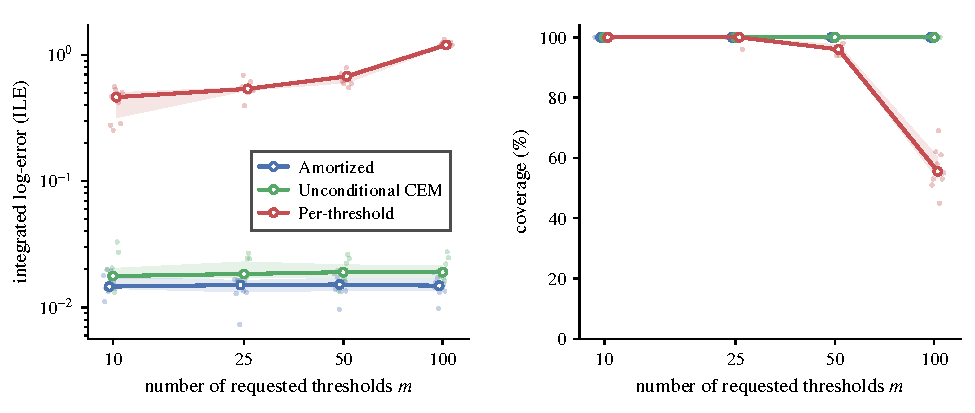
\includegraphics[width=0.9\linewidth]{figures/main/exp1_kscaling.pdf}
    \caption{
    Effect of the number of requested thresholds under a fixed budget of \(25{,}000\) robustness evaluations. Left: integrated log-error. Right: coverage. Lines show medians over 10 seeds, points show individual seeds, and shading shows the interquartile range. The amortized and unconditional CEM methods use one adaptive run for the full grid. The per-threshold baseline splits the same budget across \(m\) independently fitted proposals.
    }
    \label{fig:amortization}
\end{figure}

In contrast, the per-threshold baseline degrades as the same total budget is divided among more independently fitted proposals: median ILE increases from $0.463$ at $m=10$ to $0.539$, $0.677$, and $1.20$ at $m=25$, $50$, and $100$, respectively. Median coverage is 100\%, 100\%, 96\%, and 55.5\% over the same values of $m$. At $m=100$, individual per-threshold runs produce finite positive estimates for only 45--69\% of the requested thresholds.

The result is not explained solely by missing estimates. At $m=10$, all three methods achieve complete coverage, yet the per-threshold baseline already has substantially larger ILE. As $m$ increases, per-threshold refitting incurs both larger estimation error and, eventually, loss of coverage. By contrast, both shared-run methods maintain nearly constant curve-level error as the threshold grid becomes denser. This supports the central amortization claim: reusing a single adaptive run across thresholds avoids repeatedly spending the simulation and fitting budget on separate proposals.

The unconditional CEM baseline performs similarly to the robustness-conditioned method in this unimodal benchmark, with median ILE only about $1.2$--$1.3$ times larger across the four grids and complete coverage throughout. Thus, this experiment does not isolate a substantial benefit from robustness conditioning itself. Rather, it shows that the dominant advantage in this setting comes from sharing adaptive proposal learning and samples across requested thresholds.

% Section 5.3
% --------------------------------------------------------------
\subsection{Failure Geometry and Discovery Limits}
\label{sec:geometry-results}

We next test whether amortization remains effective when the failure region contains little directional structure. We use an isotropic shell benchmark
\[
    \rho(x) = r_c - \lVert x\rVert_2,
    \qquad
    x \sim \mathcal{N}(0,I_d)
\]
with failure defined by $\rho(x)\leq\gamma$. The corresponding failure probability is available in closed form from the upper tail of a $\chi^2_d$ distribution. We evaluate 16 thresholds whose true failure probabilities range from $10^{-3}$ to $10^{-6}$ at dimensions $d\in\{2,20\}$ and nominal budgets $B\in\{25{,}000,50{,}000\}$.

We compare the amortized method against an oracle-tuned per-threshold importance-sampling baseline and oracle-tuned adaptive multilevel splitting (AMS). Both baselines select their hyperparameters using the ground-truth failure probabilities, which the amortized method never observes, and all evaluations spent during that selection are charged to the baseline. The actual budgets therefore differ substantially across methods: at nominal budget $25{,}000$, the amortized method uses $25{,}000$ evaluations, the per-threshold oracle uses $72{,}000$, and AMS uses $168{,}261$. At nominal budget $50{,}000$, these totals are $50{,}000$, $145{,}600$, and $338{,}097$. At $d=20$, the corresponding AMS totals are $174{,}498$ and $351{,}275$. We therefore interpret this experiment as a test of discovery and robustness to failure geometry rather than as a matched-budget comparison.

\begin{figure}[ht!]
    \centering
    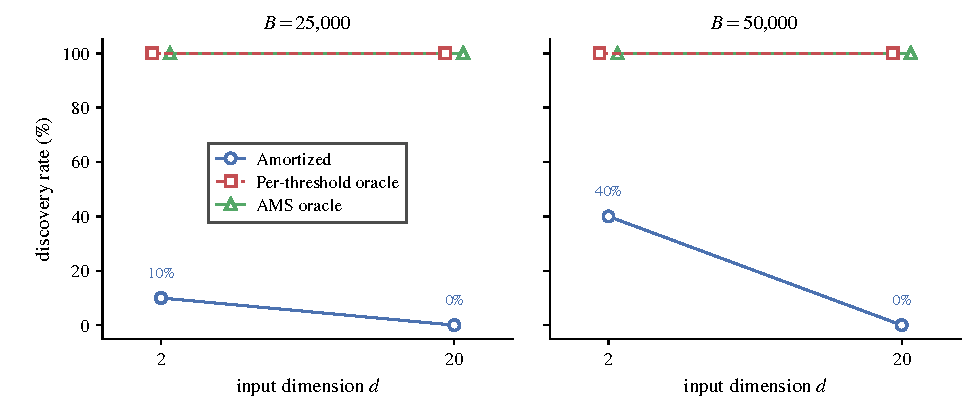
\includegraphics[width=0.9\linewidth]{figures/main/exp2_shell_discovery.pdf}
    \caption{
    Discovery on the radial-shell benchmark. Discovery rate is the fraction of 10 seeds with at least one finite positive estimate on the 16-threshold grid. The amortized method reaches the grid in 1/10 and 4/10 seeds at \(d=2\) for \(B=25{,}000\) and \(50{,}000\), and in 0/10 seeds at \(d=20\) for both budgets. Both oracle-tuned baselines succeed in all seeds. \(B\) is the nominal budget.
    }
    \label{fig:shell-discovery}
\end{figure}

\paragraph{Discovery dominates performance.}
As shown in \cref{fig:shell-discovery}, discovery is the dominant limitation for the amortized method on the shell benchmark. At $d=2$, it produces at least one finite positive estimate in only 1 of 10 seeds at $B=25{,}000$ and 4 of 10 seeds at $B=50{,}000$. The successful seed at the lower budget covers 81.25\% of the grid, while coverage among the four successful seeds at the larger budget ranges from 18.75\% to 100\%. At $d=20$, the amortized method produces no finite positive estimate in any seed at either budget. Consequently, its aggregate ILE in the zero-coverage cells is determined entirely by the $1/B$ missing-estimate convention and should not be interpreted as curve-estimation error. This reflects the adaptive schedule rather than an absence of samples in the evaluation region: in every cell all ten seeds generated draws at or below the loosest grid threshold, while the schedule reached that threshold in only $1$, $4$, $0$, and $0$ seeds, respectively (\cref{app:reproducibility}).

\begin{table}[ht!]
    \centering
    \small
    \caption{
    Radial-shell results over 10 seeds. \(B\) is the nominal budget and “Evals” the median actual count including oracle tuning. Coverage is the median fraction of the 16-point grid with a finite positive estimate. “Any” counts seeds with at least one estimate, and “$\mathrm{ILE}\mid\mathrm{any}$” is the median ILE over those seeds. Daggers mark zero-median-coverage rows, where primary ILE is dominated by the $1/B_{\mathrm{actual}}$ missing-estimate convention.
    }
    \label{tab:shell-results}
    \begin{tabular}{@{}cc l r r r c r@{}}
        \toprule
        $d$ & $B$ & Method
        & Evals
        & ILE
        & Coverage
        & Any
        & $\mathrm{ILE}\mid\mathrm{any}$ \\
        \midrule

        2 & 25k
          & Amortized
          & 25,000
          & $1.843^{\dagger}$
          & 0\%
          & 1/10
          & 0.909 \\

        2 & 25k
          & Per-threshold oracle
          & 72,000
          & 1.157
          & 84.4\%
          & 10/10
          & 1.157 \\

        2 & 25k
          & AMS oracle
          & 168,261
          & 0.072
          & 100\%
          & 10/10
          & 0.072 \\

        \addlinespace

        2 & 50k
          & Amortized
          & 50,000
          & $1.871^{\dagger}$
          & 0\%
          & 4/10
          & 0.871 \\

        2 & 50k
          & Per-threshold oracle
          & 145,600
          & 0.804
          & 100\%
          & 10/10
          & 0.804 \\
          
        2 & 50k
          & AMS oracle
          & 338,097
          & 0.083
          & 100\%
          & 10/10
          & 0.083 \\

        \midrule

        20 & 25k
           & Amortized
           & 25,000
           & $1.843^{\dagger}$
           & 0\%
           & 0/10
           & -- \\

        20 & 25k
           & Per-threshold oracle
           & 72,000
           & 8.320
           & 100\%
           & 10/10
           & 8.320 \\

        20 & 25k
           & AMS oracle
           & 174,498
           & 0.172
           & 100\%
           & 10/10
           & 0.172 \\

        \addlinespace

        20 & 50k
           & Amortized
           & 50,000
           & $1.871^{\dagger}$
           & 0\%
           & 0/10
           & -- \\

        20 & 50k
           & Per-threshold oracle
           & 145,600
           & 4.841
           & 100\%
           & 10/10
           & 4.841 \\

        20 & 50k
           & AMS oracle
           & 351,275
           & 0.146
           & 100\%
           & 10/10
           & 0.146 \\

        \bottomrule
    \end{tabular}
\end{table}

\paragraph{Accuracy conditional on discovery.}
Conditional on producing at least one estimate, the low-dimensional results are substantially less adverse. At $d=2$, the amortized method has median conditional ILE $0.909$ at $B=25{,}000$---supported by the single seed that reached the grid---and $0.871$ at $B=50{,}000$, over the four seeds that reached it. The oracle-tuned per-threshold baselines attain $1.157$ and $0.804$ on the same missing-estimate convention over all ten seeds and at $2.9$ times the evaluation budget. These figures rest on very few amortized-method seeds and an unequal budget, so we read them only as evidence that estimation does not collapse once the region is reached, rather than as a performance comparison. The principal limitation in this experiment is therefore failure discovery, not estimation conditional on discovery.

\paragraph{Higher-dimensional shell.}
The discovery limitation becomes decisive at $d=20$. The amortized method has zero coverage in every seed at both budgets, whereas AMS maintains complete coverage across all 10 seeds. AMS attains median ILE $0.172$ at nominal budget $25{,}000$ and $0.146$ at nominal budget $50{,}000$. The oracle-tuned per-threshold baseline has median coverage of 100\% at $d=20$, but with median ILE $8.32$ and $4.84$, respectively.

The shell benchmark therefore identifies a scope boundary for amortized proposal learning. Sharing information across robustness levels is useful only after the adaptive sampler has discovered the relevant failure structure. For an extended isotropic failure region, that discovery step can itself dominate the finite-budget problem. Increasing the budget improves discovery at $d=2$, from 1 of 10 to 4 of 10 seeds, but does not produce discovery at $d=20$ in this experiment. We do not read this as evidence that the conditional mixture family cannot represent a shell at a fixed threshold. The experiment does not test that question because discovery fails first.

% Section 5.4
% --------------------------------------------------------------
\subsection{When Does Robustness Conditioning Help?}
\label{sec:conditioning-results}

We next isolate the role of robustness conditioning using a two-dimensional multimodal tail benchmark
\[
    \rho(x)
    =
    \min\!\left(c_1-x_1,\; c_2-x_2^2\right),
    \qquad
    x\sim\mathcal N(0,I_2)
\]
with $c_1=5.5$ and $c_2\in\{16,18,20,23\}$. Failure is defined by $\rho(x)\leq 0$. The corresponding probability is available in closed form,
\[
    P(\rho(X)\leq 0)
    =
    P_1 + P_2 - P_1P_2,
\]
where
\[
    P_1=\Phi(-c_1),
    \qquad
    P_2=2\Phi(-\sqrt{c_2}).
\]
Changing $c_2$ changes the relative contribution of the two failure mechanisms, providing a setting in which the important input modes vary with robustness.

We compare the full robustness-conditioned proposal with an unconditional cross-entropy baseline using three-component Gaussian-mixture proposals. Both methods use exactly $80{,}000$ robustness evaluations per seed and each setting is repeated over 10 seeds. The conditioned method fits on the accumulated sample buffer, whereas the unconditional baseline fits on elites from the current batch. Thus, the comparison measures the performance of the full conditioned method against the unconditional baseline rather than isolating conditioning alone. Because this experiment estimates a single failure probability at $\gamma=0$, we report $\widehat P/P_{\mathrm{true}}$ directly rather than ILE.

\begin{figure}[ht!]
    \centering
    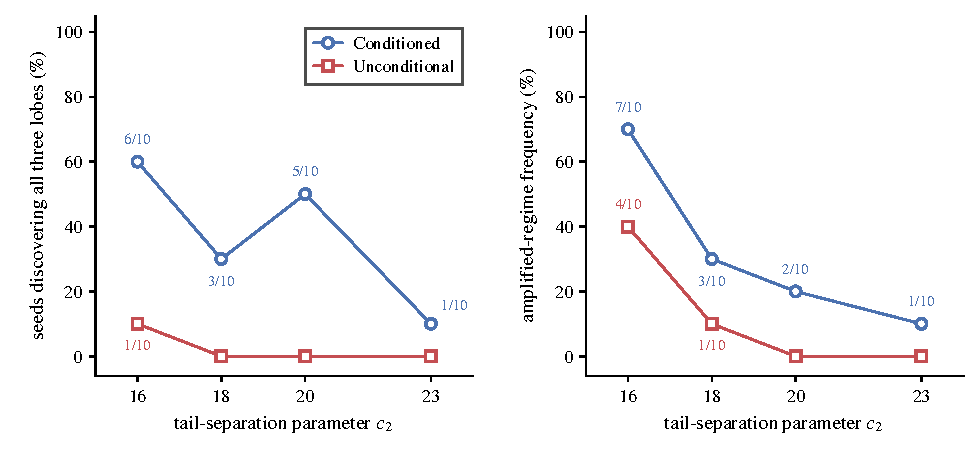
\includegraphics[width=0.9\linewidth]{figures/main/exp3_conditioning_modes.pdf}
    \caption{
    Effect of robustness conditioning on failure-mode discovery in the multimodal tail benchmark. Left: fraction of seeds discovering all three failure lobes. Right: fraction reaching the amplified regime, where the two \(x_2\) lobes recover more than \(10\%\) of the true failure probability. Criteria are defined in \cref{app:tail-benchmark-results}. The conditioned method more often discovers and retains the \(x_2\) modes. All 80 runs underestimate the true failure probability. The unconditional aggregates at \(c_2=16\), \(18\), and \(23\) each include one fallback-assisted run.
    }
    \label{fig:conditioning-modes}
    \vspace{-0.2cm}
\end{figure}

\paragraph{The conditioned method improves mode discovery under the single-draw criterion.}
As shown in \cref{fig:conditioning-modes}, the conditioned method discovers all three failure lobes more often than the unconditional baseline across the four values of $c_2$. The discovery counts are 6/10, 3/10, 5/10, and 1/10 for $c_2=16,18,20,$ and $23$, respectively, compared with 1/10, 0/10, 0/10, and 0/10 for the unconditional baseline. The run's own deterministic regime classification, defined exactly in \cref{app:tail-benchmark-results}, shows a difference in the same direction but of smaller size. Conditioned runs reach the amplified regime---recovering more than \(10\%\) of the true failure probability from the two \(x_2\) lobes---in 7, 3, 2, and 1 seeds across the four settings, versus 4, 1, 0, and 0 for the unconditional baseline. Unconditional runs are increasingly locked out of both \(x_2\) lobes, as \(c_2\) grows, with 2, 5, 7, and 9 of 10 seeds locked across the four settings.

\paragraph{Effect on probability estimation.}
The conditioned method also tends to recover more probability mass from the relevant rare-event modes, but the effect is highly variable across seeds. Its median $\widehat P/P_{\mathrm{true}}$ is $0.436$, $0.00365$, $0.00237$, and $0.0107$ for $c_2=16,18,20,$ and $23$, respectively. The corresponding unconditional medians are $0.00837$, $8.87\times10^{-4}$, $1.82\times10^{-3}$, and $8.48\times10^{-3}$. At the same time, several conditioned cells span orders of magnitude across seeds. For example, at $c_2=18$ the ratio ranges from $7.7\times10^{-4}$ to $0.83$. Both methods remain far below the target throughout: no seed in the 80 runs produces an estimate above the true probability, the best single run reaches $\widehat P/P_{\mathrm{true}}=0.99$, and in seven of the eight cells the median estimate is low by a factor of between $94$ and $1{,}130$.

The apparent improvement in the ratio at larger $c_2$ is a denominator effect rather than a gain in accuracy: the median absolute estimate changes by less than a factor of $1.5$ across $c_2=18,20,23$ ($1.96\times10^{-8}$, $1.41\times10^{-8}$, and $1.39\times10^{-8}$ for the unconditional method) while the true probability falls by a factor of $13.5$ over the same range. In a safety-validation setting, these finite-budget estimates are systematically anti-conservative in this experiment: $\widehat P<P_{\mathrm{true}}$ in all 80 runs, so using the realized estimates directly would understate the true failure probability. The per-lobe diagnostics indicate that this shortfall is associated with failing to recover probability mass from the dominant $x_2$ failure modes. Thus, conditioning improves access to changing failure modes but does not make the resulting estimator uniformly accurate.

The unconditional baseline requires an implementation caveat. One run in each of the $c_2=16$, $18$, and $23$ unconditional cells completed only after a degenerate-fit fallback was added to the unconditional expectation-maximization Gaussian mixture model (EMGMM) fitting path. All other runs are clean. None of these three runs discovers all three lobes or reaches the amplified regime, and excluding them changes the unconditional median $\widehat P/P_{\mathrm{true}}$ only modestly: from $0.00837$ to $0.00898$ at $c_2=16$, from $8.87\times10^{-4}$ to $1.14\times10^{-3}$ at $c_2=18$, and from $8.48\times10^{-3}$ to $8.49\times10^{-3}$ at $c_2=23$. We therefore use the full 10-seed aggregates for reporting.

Overall, the conditioned method discovers changing failure modes more consistently than the unconditional baseline. It also reaches the amplified regime more often overall, in 13 versus 5 of 40 seeds, but this gap is smaller than the discovery gap. Run-level regime labels depend on individual adaptive trajectories, so differences of a single seed, such as 1/10 versus 0/10, should not be interpreted. Part of its advantage in retaining previously discovered modes may come from fitting on the accumulated sample buffer rather than the current batch alone. However, this difference cannot explain cases in which the conditioned method discovers a mode that the unconditional baseline never encounters. The results therefore support the use of robustness-conditioned proposals for multimodal rare-event problems, while not isolating conditioning as the sole source of the observed improvement.

% Section 5.5
% --------------------------------------------------------------
\subsection{High-Dimensional Closed-Loop Driving}
\label{sec:driving-results}

Finally, we evaluate the method on a closed-loop autonomous-driving problem with a $150$-dimensional disturbance input. The scenario contains 30 disturbance steps with five channels per step, and robustness is defined from the running maximum point-of-closest-approach reward. We evaluate an eight-point threshold grid from $\gamma=0.434$ to the target $\gamma=0$, using a $26$-million-rollout reference curve. The reference is a finite Monte Carlo estimate: its relative standard error ranges from $0.21\%$ at $\gamma=0.434$ to $3.5\%$ at the two rarest grid points. The reference contains the same $808$ observed events at $\gamma=0.08$ and $\gamma=0$, although the two thresholds are mathematically distinct under the simulator definition.

\begin{table}[ht!]
\centering
\caption{
    High-dimensional closed-loop driving results over 10 seeds. Evals is the charged simulator-evaluation count including oracle tuning; for AMS, the median is shown, with range \(101{,}024\)--\(125{,}936\). Coverage is the median fraction of the eight-threshold grid with a finite positive estimate, and Any/Zero count seeds with at least one/no estimate. ILE uses the \(1/B_{\mathrm{actual}}\) missing-estimate convention.
    }
\label{tab:driving-results}
\begin{tabular}{@{}lrrrrr@{}}
\toprule
Method & Evals & ILE & Coverage & Any & Zero \\
\midrule
Amortized     & 25,000  & 0.484 & 100\%   & 10/10 & 0/10 \\
Per-threshold & 48,000  & 3.498 & 68.75\% & 10/10 & 0/10 \\
AMS           & 115,018 & 0.465 & 87.5\%  & 10/10 & 0/10 \\
\bottomrule
\end{tabular}
\end{table}

The amortized proposal uses a two-component low-rank-plus-diagonal conditional mixture with rank 10 and a $10\%$ defensive nominal component. All three methods are evaluated over 10 seeds. Both baselines use the reference probabilities during selection, which the amortized method never observes, and all selection costs are charged in full. The amortized method uses \(25{,}000\) simulator evaluations per seed, compared with \(48{,}000\) for the per-threshold baseline. AMS evaluates all six oracle configurations and uses a median of \(115{,}018\) charged evaluations per seed, with a range of \(101{,}024\)--\(125{,}936\). The per-threshold baseline reports, at each threshold, whichever of its two candidate estimates is closer to the reference probability. The AMS baseline selects the configuration with the smallest median relative error against the reference.

\paragraph{The amortized proposal estimates the full threshold grid from a single adaptive run.}
As shown in \cref{tab:driving-results}, the amortized method produces a finite positive estimate at every evaluation threshold in all 10 seeds, giving median coverage of \(100\%\) and median ILE \(0.484\). Its adaptive schedule nevertheless does not reach the target threshold: the minimum adaptive threshold has median \(0.362\), with a range from \(0.305\) to \(0.369\), and the schedule reaches \(\gamma=0\) in no seed. Sampling reaches the target region in every seed, with \(36\) to \(66\) of the \(25{,}000\) draws at or below \(\gamma=0\), all at the simulator's collision value. Thus, schedule reach and estimator availability are distinct in this experiment. The pooled estimator can evaluate thresholds below the terminal adaptive threshold using samples collected from the sequence of fitted proposals (\cref{app:high-diagnostics}).

\begin{figure}[ht!]
    \centering
    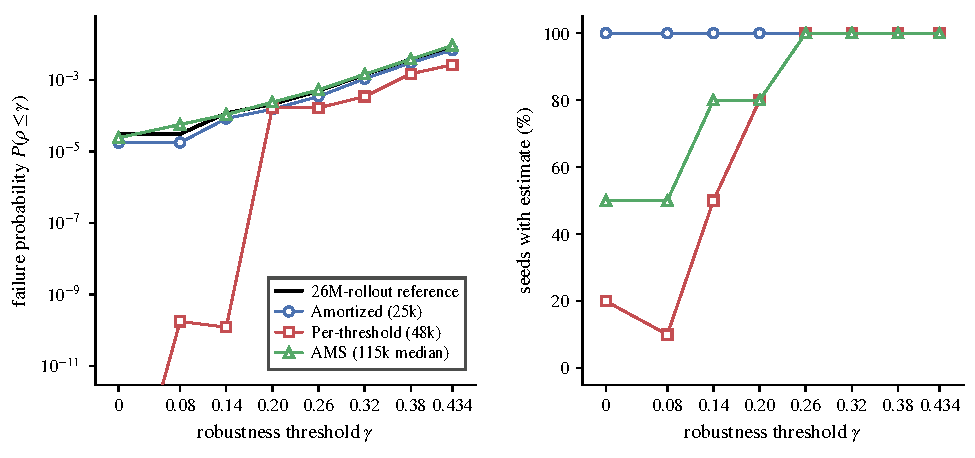
\includegraphics[width=0.9\linewidth]{figures/main/exp4_driving_curve.pdf}
    \caption{
    Failure-probability estimation on the \(150\)-dimensional closed-loop driving benchmark. Left: median finite positive estimate versus the \(26\)-million-rollout reference. The amortized method covers all thresholds in all 10 seeds, while the per-threshold baseline and AMS lose coverage in the rare tail. The reference contains the same \(808\) observed events at \(\gamma=0.08\) and \(\gamma=0\). Right: fraction of seeds with a finite positive estimate. Charged evaluation budgets are shown in the legend.
    }
    \label{fig:driving-curve}
\end{figure}

\paragraph{The amortized method achieves error comparable to AMS at substantially lower simulation cost.}
AMS attains median ILE \(0.465\), compared with \(0.484\) for the amortized method. These median errors are similar, while AMS uses a median of \(115{,}018\) charged simulator evaluations per seed, about \(4.6\) times the \(25{,}000\) evaluations used by the amortized method. AMS has median coverage of \(87.5\%\), with at least one finite positive estimate in every seed. The per-threshold baseline performs substantially worse despite using nearly twice the amortized method's simulation budget: it has median ILE \(3.50\) and median coverage \(68.75\%\). Thus, independently refitting proposals at each threshold does not recover the advantage obtained by sharing proposal learning across the curve in this problem.

\paragraph{High dimension increases weight concentration without preventing full-curve estimation.}
For the amortized method, the effective-sample-size fraction of the proposal-fitting weights has median \(0.117\), close to the lower bound of approximately \(\eta=0.1\) implied by the defensive mixture's weight bound. The effective-sample-size fraction of the pooled balance-MIS estimator weights, computed over the re-indexed samples with \(\rho\leq0.434\), has median \(0.0256\), indicating substantial concentration in the estimator weights. At the target threshold, the absolute effective sample size has median \(5.8\). Despite this concentration, every seed yields a finite target-threshold estimate, and the 10 target estimates lie within a factor of \(3.25\) of the reference probability. These diagnostics show that high-dimensional proposal fitting remains difficult, but in this experiment the resulting weight concentration does not prevent estimation across the full requested threshold grid.

The driving experiment therefore provides a high-dimensional test of amortized rare-event estimation under closed-loop dynamics. The amortized method achieves median curve-estimation error comparable to oracle-tuned AMS while using substantially fewer simulator evaluations, and it substantially outperforms independently refitted per-threshold proposals. The adaptive schedule itself does not descend to the target threshold, but the samples collected across the adaptive run are sufficient to estimate the full threshold grid. These results support amortizing proposal learning across thresholds even in a \(150\)-dimensional setting, while also showing that estimator-weight concentration remains an important limitation at the rarest thresholds.

% ==============================================================
% 6. CONCLUSION
% ==============================================================
\section{Conclusion}
\label{sec:conclusion}

We introduced an amortized approach to rare-event estimation that learns a single proposal model and reuses it across a family of nested failure thresholds. Rather than fitting an independent input proposal for each threshold, the method models the relationship between system inputs and robustness and constructs threshold-specific proposals by truncating the learned robustness marginal. A single adaptive run can therefore support estimation of an entire failure-probability curve.

The experiments show that this amortization can provide a substantial finite-budget benefit when the relevant failure structure is discovered and shared across thresholds. On the unimodal benchmark, both the robustness-conditioned method and an unconditional adaptive baseline maintain nearly constant error as the number of requested thresholds increases from 10 to 100 under a fixed total simulation budget, while independently refitted per-threshold proposals become progressively less accurate and eventually lose coverage. The unconditional baseline performs comparably to the robustness-conditioned method, indicating that the dominant benefit in this setting comes from reusing simulation and proposal-fitting effort across thresholds rather than from robustness conditioning itself.

The experiments also identify an important limitation: shared proposal learning cannot exploit failure structure that the adaptive sampler does not discover. On the radial-shell benchmark, the amortized method reaches the evaluation region in only 1 of 10 seeds at a nominal budget of $25{,}000$ and 4 of 10 seeds at $50{,}000$ in two dimensions, and in no seeds at either budget in 20 dimensions. Conditional on discovery in the two-dimensional case, however, its curve-estimation error is comparable to the per-threshold baseline. This separates two sources of difficulty: discovering the relevant rare-event region and estimating probabilities once that region has been reached.

The multimodal tail benchmark further examines the role of robustness conditioning, although it does not isolate conditioning because the conditioned method also fits on its accumulated sample buffer. Across all four settings, the conditioned proposal discovers all three failure modes more often than the unconditional baseline; it also amplifies secondary modes more often overall, although by a smaller margin. The resulting probability estimates nevertheless remain highly variable across seeds. Robustness conditioning is therefore most useful when the important input modes change systematically with robustness and those modes are observed during adaptation. It does not by itself solve mode discovery.

The high-dimensional driving experiment shows that amortized proposal learning can remain effective even when the input space is large. The amortized method achieves error comparable to oracle-tuned AMS using $25{,}000$ simulator evaluations, versus a median of $115{,}018$ for AMS, and substantially outperforms independently refitted per-threshold proposals. Concentrated estimator weights in the rare tail nevertheless indicate that high-dimensional rare-event estimation remains challenging even when amortization is effective.

Taken together, these results characterize amortized proposal learning as a finite-budget strategy rather than a uniformly superior rare-event estimator. Its benefit is largest when failure structure is shared across robustness levels and can be discovered with a common adaptive run. The experiments also show that discovery, multimodality, and estimator-weight concentration remain important limitations. Future work should focus on improved mode and direction discovery, adaptive selection of robustness levels, and richer conditional proposal families with tractable marginal densities. Evaluating these ideas in higher-fidelity autonomous-system simulators will test whether reducing repeated proposal fitting translates into lower validation cost when simulation dominates computation.

% ==== END MAIN TEXT ====

% Acknowledgments
% ==============================================================
\acks{This work was supported by the National Science Foundation (NSF) Graduate Research Fellowship under Grant No. DGE-2146755. Any opinions, findings, or conclusions expressed here do not reflect the views of the NSF. The authors have no competing interests to declare.}

% ==============================================================
% BIBLIOGRAPHY
% ==============================================================
\vskip 0.2in
\bibliography{references}

% ==============================================================
% APPENDIX
% ==============================================================
\newpage
\appendix

% ==============================================================
% A. PROOFS AND THEORETICAL DETAILS
% ==============================================================
\section{Proofs and Theoretical Details}
\label{app:theory}

This appendix provides proofs and additional details for the theoretical results in \cref{sec:method}.

% Section A.1
% --------------------------------------------------------------
\subsection{Failure-Set Nesting}
\label{app:failure-nesting}

For thresholds $\gamma_1<\gamma_2$, the corresponding failure sets are nested as
\[
    \{x:\rho(x)\leq\gamma_1\}
    \subseteq
    \{x:\rho(x)\leq\gamma_2\}.
\]
The associated conditional input distributions satisfy
\[
    p(x\mid\rho(x)\leq\gamma_1)
    =
    \frac{
        p(x\mid\rho(x)\leq\gamma_2)
        \mathds{1}\{\rho(x)\leq\gamma_1\}
    }{
        P\!\left(
            \rho(X)\leq\gamma_1
            \mid
            \rho(X)\leq\gamma_2
        \right)
    }.
\]

\begin{proof}
Starting from the right-hand side,
\[
\begin{aligned}
\frac{
    p(x\mid\rho(x)\leq\gamma_2)
    \mathds{1}\{\rho(x)\leq\gamma_1\}
}{
    P(
        \rho(X)\leq\gamma_1
        \mid
        \rho(X)\leq\gamma_2
    )
}
&=
\frac{
    p(x)
    \mathds{1}\{\rho(x)\leq\gamma_2\}
    \mathds{1}\{\rho(x)\leq\gamma_1\}
}{
    P(\rho(X)\leq\gamma_2)
    P(
        \rho(X)\leq\gamma_1
        \mid
        \rho(X)\leq\gamma_2
    )
}.
\end{aligned}
\]
Because $\gamma_1<\gamma_2$,
\[
    \mathds{1}\{\rho(x)\leq\gamma_2\}
    \mathds{1}\{\rho(x)\leq\gamma_1\}
    =
    \mathds{1}\{\rho(x)\leq\gamma_1\}
\]
and
\[
    P(\rho(X)\leq\gamma_2)
    P(
        \rho(X)\leq\gamma_1
        \mid
        \rho(X)\leq\gamma_2
    )
    =
    P(\rho(X)\leq\gamma_1).
\]
Therefore,
\[
    \frac{
        p(x)\mathds{1}\{\rho(x)\leq\gamma_1\}
    }{
        P(\rho(X)\leq\gamma_1)
    }
    =
    p(x\mid\rho(x)\leq\gamma_1),
\]
which proves the result.
\end{proof}

% Section A.2
% --------------------------------------------------------------
\subsection{Smoothed Observation Model}
\label{app:smoothed-observation}

Because $R=\rho(X)$ is deterministic given $X$, the joint distribution of $(X,R)$ is supported on the graph $\{(x,\rho(x))\}$ and is singular with respect to Lebesgue measure on $\mathcal X\times\mathbb R$. For $\sigma>0$, define the noisy robustness observation
\[
    \tilde R
    =
    \rho(X)+\varepsilon,
    \qquad
    \varepsilon\sim\mathcal N(0,\sigma^2).
\]
Its joint density with $X$ is
\[
    \tilde p_\sigma(x,r)
    =
    p(x)k_\sigma(r-\rho(x)),
\]
where $k_\sigma$ is the Gaussian density with standard deviation $\sigma$.

\paragraph{Well-posedness.}
For every $\sigma>0$, $\tilde p_\sigma$ is an absolutely continuous probability density on $\mathcal X\times\mathbb R$. Moreover, its marginal density over $x$ is the nominal input density $p(x)$.
\vspace{0.3cm}

\begin{proof}
Nonnegativity follows from nonnegativity of $p$ and $k_\sigma$. Integrating over both variables gives
\[
\begin{aligned}
    \int_{\mathcal X}\int_{\mathbb R}
    \tilde p_\sigma(x,r)\,dr\,dx
    &=
    \int_{\mathcal X}
    p(x)
    \left[
        \int_{\mathbb R}
        k_\sigma(r-\rho(x))\,dr
    \right]dx \\
    &=
    \int_{\mathcal X}p(x)\,dx \\
    &=1.
\end{aligned}
\]
Similarly,
\[
    \int_{\mathbb R}
    \tilde p_\sigma(x,r)\,dr
    =
    p(x)
\]
because the Gaussian kernel integrates to one.
\end{proof}

Marginalizing the smoothed density over the sublevel set $r\leq\gamma$ gives
\[
\begin{aligned}
    \int_{-\infty}^{\gamma}
    \tilde p_\sigma(x,r)\,dr
    &=
    p(x)
    \int_{-\infty}^{\gamma}
    k_\sigma(r-\rho(x))\,dr \\
    &=
    p(x)
    \Phi\!\left(
        \frac{\gamma-\rho(x)}{\sigma}
    \right)
\end{aligned}
\]
where $\Phi$ is the standard normal cumulative distribution function. Thus, smoothing replaces the hard indicator $\mathds{1}\{\rho(x)\leq\gamma\}$ with the probit factor
\[
    \Phi\!\left(
        \frac{\gamma-\rho(x)}{\sigma}
    \right).
\]
For every $x$ such that $\rho(x)\neq\gamma$, this factor converges to $\mathds{1}\{\rho(x)\leq\gamma\}$ as $\sigma\to0$.

% Section A.3
% --------------------------------------------------------------
\subsection{Convergence of the Smoothed Target}
\label{app:smoothing-convergence}

\begin{proposition}
\label{prop:smoothing-convergence}
Fix a threshold $\gamma$ such that
\[
    F_\rho(\gamma)
    =
    P(R\leq\gamma)
    >
    0.
\]
Assume there exists $\delta>0$ such that $R=\rho(X)$ admits a density $f_\rho$ on $I_\delta:=(\gamma-\delta,\gamma+\delta)$ that is bounded on $I_\delta$ and continuous at $\gamma$. No global density, boundedness, or continuity of $f_\rho$ is assumed. Outside $I_\delta$, the distribution of $R$ is arbitrary.

Define
\[
    h_\sigma(r)
    =
    \Phi\!\left(
        \frac{\gamma-r}{\sigma}
    \right),
    \qquad
    Z_\sigma
    =
    \mathbb E[h_\sigma(R)].
\]
The normalized smoothed target is
\[
    q_\sigma^\gamma(x)
    =
    \frac{
        p(x)h_\sigma(\rho(x))
    }{
        Z_\sigma
    },
\]
while the hard conditional target is
\[
    q^{*\gamma}(x)
    =
    \frac{
        p(x)\mathds{1}\{\rho(x)\leq\gamma\}
    }{
        F_\rho(\gamma)
    }.
\]
Then, as $\sigma\to0$,
\[
    \operatorname{TV}
    \left(
        q_\sigma^\gamma,
        q^{*\gamma}
    \right)
    =
    \frac{\sigma}{\sqrt{2\pi}}
    \lambda_\rho(\gamma)
    +
    o(\sigma),
    \qquad
    \lambda_\rho(\gamma)
    =
    \frac{
        f_\rho(\gamma)
    }{
        F_\rho(\gamma)
    }.
\]
Thus, if $f_\rho(\gamma)>0$,
\[
    \operatorname{TV}
    \left(
        q_\sigma^\gamma,
        q^{*\gamma}
    \right)
    =
    \frac{\sigma}{\sqrt{2\pi}}
    \lambda_\rho(\gamma)
    \bigl(1+o(1)\bigr).
\]
If $f_\rho(\gamma)=0$, the conclusion is instead
\[
    \operatorname{TV}
    \left(
        q_\sigma^\gamma,
        q^{*\gamma}
    \right)
    =
    o(\sigma).
\]
The multiplicative form does not apply in this case: whenever $P(R>\gamma)>0$, $q_\sigma^\gamma$ assigns positive mass above $\gamma$ for every $\sigma>0$, whereas $q^{*\gamma}$ does not.
\end{proposition}

\vspace{0.3cm}
\begin{proof}
Write $F=F_\rho(\gamma)$ and
\[
    H_\gamma(r)
    =
    \mathds{1}\{r\leq\gamma\}.
\]
Because both targets are absolutely continuous with respect to the nominal distribution of $X$, with Radon--Nikodym derivatives depending on $x$ only through $\rho(x)$,
\[
    \operatorname{TV}
    \left(
        q_\sigma^\gamma,
        q^{*\gamma}
    \right)
    =
    \frac{1}{2}
    \mathbb E
    \left|
        \frac{h_\sigma(R)}{Z_\sigma}
        -
        \frac{H_\gamma(R)}{F}
    \right|.
\]
Moreover,
\begin{equation}
\label{eq:tv-normalization-split}
    \left|
        2\operatorname{TV}
        \left(
            q_\sigma^\gamma,
            q^{*\gamma}
        \right)
        -
        \frac{1}{F}
        \mathbb E
        \left|
            h_\sigma(R)-H_\gamma(R)
        \right|
    \right|
    \leq
    \frac{|Z_\sigma-F|}{F}.
\end{equation}
It therefore suffices to expand the unnormalized $L^1$ error and show that $Z_\sigma-F=o(\sigma)$.

Let
\[
    g(u)
    =
    \Phi(-u)
    -
    \mathds{1}\{u\leq0\},
\]
so that
\[
    h_\sigma(r)-H_\gamma(r)
    =
    g\!\left(
        \frac{r-\gamma}{\sigma}
    \right).
\]
The kernel satisfies
\[
    |g(u)|
    =
    \Phi(-|u|),
    \qquad
    \int_{\mathbb R}|g(u)|\,du
    =
    \sqrt{\frac{2}{\pi}},
\]
and, by antisymmetry,
\[
    \int_{-A}^{A}g(u)\,du
    =
    0
    \qquad
    \text{for every }A>0.
\]

For any measurable $\psi$ with $|\psi(u)|\leq\Phi(-|u|)$, split the expectation into $R\in I_\delta$ and $R\notin I_\delta$. On $I_\delta$, the change of variables $r=\gamma+\sigma u$ gives
\[
    \mathbb E
    \left[
        \psi\!\left(
            \frac{R-\gamma}{\sigma}
        \right)
        \mathds{1}\{R\in I_\delta\}
    \right]
    =
    \sigma
    \int_{|u|<\delta/\sigma}
    \psi(u)
    f_\rho(\gamma+\sigma u)\,du.
\]
Continuity of $f_\rho$ at $\gamma$, boundedness on $I_\delta$, and integrability of $\psi$ then give
\[
    \sigma
    \int_{|u|<\delta/\sigma}
    \psi(u)f_\rho(\gamma+\sigma u)\,du
    =
    \sigma f_\rho(\gamma)
    \int_{|u|<\delta/\sigma}\psi(u)\,du
    +
    o(\sigma).
\]
Outside $I_\delta$,
\[
    \left|
        \psi\!\left(
            \frac{R-\gamma}{\sigma}
        \right)
    \right|
    \leq
    \Phi(-\delta/\sigma),
\]
so the tail contribution is superpolynomially small.

Taking $\psi=|g|$ therefore gives
\[
    \mathbb E
    \left|
        h_\sigma(R)-H_\gamma(R)
    \right|
    =
    \sigma f_\rho(\gamma)
    \sqrt{\frac{2}{\pi}}
    +
    o(\sigma).
\]
Taking $\psi=g$ and using $\int_{-\delta/\sigma}^{\delta/\sigma}g(u)\,du=0$ gives
\[
    Z_\sigma
    =
    F_\rho(\gamma)
    +
    o(\sigma).
\]
Substituting these expressions into \eqref{eq:tv-normalization-split} gives
\[
    \operatorname{TV}
    \left(
        q_\sigma^\gamma,
        q^{*\gamma}
    \right)
    =
    \frac{\sigma f_\rho(\gamma)}
         {\sqrt{2\pi}F_\rho(\gamma)}
    +
    o(\sigma)
    =
    \frac{\sigma}{\sqrt{2\pi}}
    \lambda_\rho(\gamma)
    +
    o(\sigma).
\]
The stated cases for $f_\rho(\gamma)>0$ and $f_\rho(\gamma)=0$ follow immediately.
\end{proof}

This is a fixed-threshold statement about the target distribution. It does not establish convergence of a fitted conditional proposal or justify a particular adaptive schedule for $\sigma$; proposal approximation error is separate from the smoothing error characterized above.

% Section A.4
% --------------------------------------------------------------
\subsection{Unbiasedness Under Adaptive Proposals}
\label{app:adaptive-unbiasedness}

We next establish unbiasedness for proposal-of-origin importance sampling under adaptive proposal selection. This result applies to the batch estimator in \cref{eq:batch-is}. It does not establish unbiasedness of the adaptive balance-MIS estimator in \cref{eq:balance-mis-estimator}.

Let $\mathcal F_{k-1}$ denote the history available before iteration $k$, and suppose the proposal $q_X^{(k)}$ is $\mathcal F_{k-1}$-measurable. Conditional on this history, draw
\[
    X_{k,1},\ldots,X_{k,n_k}
    \overset{\mathrm{iid}}{\sim}
    q_X^{(k)}.
\]
For a fixed evaluation threshold $\gamma$, define
\[
    \widehat P_k(\gamma)
    =
    \frac{1}{n_k}
    \sum_{i=1}^{n_k}
    \frac{
        p(X_{k,i})
    }{
        q_X^{(k)}(X_{k,i})
    }
    \mathds{1}\{
        \rho(X_{k,i})\leq\gamma
    \}.
\]
Assume $q_X^{(k)}(x)>0$ whenever $p(x)\mathds{1}\{\rho(x)\leq\gamma\}>0$, then $\mathbb E[\widehat P_k(\gamma)\mid\mathcal F_{k-1}]=P(\rho(X)\leq\gamma).$
\vspace{0.3cm}

\begin{proof}
Conditional on $\mathcal F_{k-1}$, the proposal $q_X^{(k)}$ is fixed. Therefore, for each sample,
\[
\begin{aligned}
    &
    \mathbb E
    \left[
        \frac{
            p(X_{k,i})
        }{
            q_X^{(k)}(X_{k,i})
        }
        \mathds{1}\{
            \rho(X_{k,i})\leq\gamma
        \}
        \,\middle|\,
        \mathcal F_{k-1}
    \right]
    \\
    &\qquad=
    \int
    q_X^{(k)}(x)
    \frac{
        p(x)
    }{
        q_X^{(k)}(x)
    }
    \mathds{1}\{
        \rho(x)\leq\gamma
    \}\,dx \\
    &\qquad=
    P(\rho(X)\leq\gamma).
\end{aligned}
\]
Averaging over the $n_k$ samples preserves the same conditional expectation. Taking expectation over $\mathcal F_{k-1}$ then gives
\[
    \mathbb E[
        \widehat P_k(\gamma)
    ]
    =
    P(\rho(X)\leq\gamma).
\]
\end{proof}

The result also holds for any deterministic weighted average of such batch estimators whose weights do not depend on the realized samples. In particular, averaging proposal-of-origin batch estimates across adaptive iterations remains unbiased. Proposal parameters, intermediate thresholds, and other adaptation choices may depend arbitrarily on the preceding history, provided that they are fixed before drawing the current batch and the support condition above holds.

The pooled balance-MIS estimator used by the amortized method has a different dependence structure. Its denominator contains proposals fitted using earlier samples, while later proposals may themselves depend on those samples. Consequently, the standard fixed-proposal balance-heuristic argument does not directly imply unbiasedness in this adaptive setting. We therefore use balance-MIS as the pooled estimator described in \cref{sec:alg-desc} without making an unbiasedness claim for that adaptive pooled construction.

% Section A.5
% --------------------------------------------------------------
\subsection{Defensive-Mixture Variance Bound}
\label{app:defensive-bound}

Let
\[
    q_\eta(x)
    =
    (1-\eta)q_X(x)+\eta p(x),
    \qquad
    0<\eta\leq1.
\]
Because $q_\eta(x)\geq\eta p(x)$, the corresponding importance weight satisfies
\[
    w_\eta(x)
    =
    \frac{
        p(x)
    }{
        q_\eta(x)
    }
    \leq
    \frac{1}{\eta}.
\]

For the event
\(
    F_\gamma
    =
    \{x:\rho(x)\leq\gamma\},
\)
let
\(
    P_\gamma
    =
    P(X\in F_\gamma).
\)
For one draw $X\sim q_\eta$, define
\[
    Y
    =
    w_\eta(X)
    \mathds{1}\{X\in F_\gamma\}.
\]
Then
\[
\begin{aligned}
    \mathbb E_{q_\eta}[Y^2]
    &=
    \mathbb E_{q_\eta}
    \left[
        w_\eta(X)^2
        \mathds{1}\{X\in F_\gamma\}
    \right] \\
    &\leq
    \frac{1}{\eta}
    \mathbb E_{q_\eta}
    \left[
        w_\eta(X)
        \mathds{1}\{X\in F_\gamma\}
    \right] \\
    &=
    \frac{P_\gamma}{\eta}.
\end{aligned}
\]
For the ordinary importance-sampling estimator based on $M$ independent draws from $q_\eta$,
\[
    \widehat P_\eta
    =
    \frac{1}{M}
    \sum_{i=1}^{M}
    w_\eta(X_i)
    \mathds{1}\{X_i\in F_\gamma\},
\]
we therefore have
\[
\begin{aligned}
    \operatorname{Var}(\widehat P_\eta)
    &=
    \frac{1}{M}
    \operatorname{Var}(Y) \\
    &\leq
    \frac{1}{M}
    \left(
        \frac{P_\gamma}{\eta}
        -
        P_\gamma^2
    \right) \\
    &\leq
    \frac{P_\gamma}{\eta M}.
\end{aligned}
\]
Thus, the defensive component guarantees both the pointwise weight bound $w_\eta(x)\leq1/\eta$ and a finite upper bound on the variance of the single-proposal importance-sampling estimator.

% ==============================================================
% B. EXPERIMENTAL PROBLEMS
% ==============================================================
\section{Experimental Problems}
\label{app:problems}

This appendix defines the benchmark problems used in the canonical experiments and gives the corresponding reference failure probabilities where available.

% Section B.1
% --------------------------------------------------------------
\subsection{Unimodal Gaussian Benchmark}
\label{app:unimodal}

Let $X\sim\mathcal N(0,I_2)$ and define
\(
    \rho(x)
    =
    3-\min(x_1,x_2).
\)
At threshold $\gamma$, failure occurs when $\rho(x)\leq\gamma$, or equivalently when
\[
    x_1\geq3-\gamma,
    \qquad
    x_2\geq3-\gamma.
\]
Because the coordinates are independent, 
\[
    P(\rho(X)\leq\gamma) = \Phi\!\left(-(3-\gamma)\right)^2.
\]
At $\gamma=0$,
\[
    P(\rho(X)\leq0)
    =
    \Phi(-3)^2
    \approx
    1.8222\times10^{-6}.
\]

This benchmark has a single connected failure region and is used to evaluate the benefit of amortizing proposal learning as the number of requested thresholds increases.

% Section B.2
% --------------------------------------------------------------
\subsection{Radial Shell}
\label{app:shell}

Let $X\sim\mathcal N(0,I_d)$ and define $\rho(x)=r_c-\|x\|.$ Then $\rho(x)\leq\gamma$ if and only if $\|x\|\geq r_c-\gamma.$ Since
\[
    \|X\|^2\sim\chi_d^2,
\]
the failure-probability curve is
\[
    P(\rho(X)\leq\gamma)
    =
    P\!\left(
        \chi_d^2
        \geq
        (r_c-\gamma)^2
    \right).
\]

We evaluate $d\in\{2,20\}$. For each dimension, the evaluation grid contains 16 thresholds whose exact failure probabilities are logarithmically spaced from $10^{-3}$ to $10^{-6}$. The smallest threshold is $\gamma_{\min}=0.5$, and $r_c$ is chosen so that this threshold corresponds to the rarest grid point. This gives
\[
    r_c
    =
    5.756521769751461
    \qquad
    \text{for }d=2,
\]
and
\[
    r_c
    =
    8.588305201645746
    \qquad
    \text{for }d=20.
\]

Unlike the unimodal benchmark, the shell has no distinguished failure direction: equal-robustness sets are spheres. It therefore tests whether the adaptive sampler can discover an extended isotropic rare-event region rather than a localized failure mode.

% Section B.3
% --------------------------------------------------------------
\subsection{Multimodal Tail Benchmark}
\label{app:tail-race}

Let $X\sim\mathcal N(0,I_2)$ and define
\(
    \rho(x)
    =
    \min\!\left(
        c_1-x_1,\,
        c_2-x_2^2
    \right).
\)
We fix $c_1=5.5$ and evaluate \[c_2\in\{16,18,20,23\}.\]

At threshold $\gamma$, failure occurs if either $x_1\geq c_1-\gamma$ or $|x_2|\geq\sqrt{c_2-\gamma}$, for thresholds satisfying $c_2-\gamma\geq0$. Define
\[
    P_1(\gamma)
    =
    \Phi(\gamma-c_1)
\]
and
\[
    P_2(\gamma)
    =
    2\Phi\!\left(
        -\sqrt{c_2-\gamma}
    \right).
\]
By independence,
\[
    P(\rho(X)\leq\gamma)
    =
    P_1(\gamma)
    +
    P_2(\gamma)
    -
    P_1(\gamma)P_2(\gamma).
\]

At the target threshold $\gamma=0$, the four settings have failure probabilities
\[
\begin{aligned}
    c_2=16 &: \quad 6.3361\times10^{-5},\\
    c_2=18 &: \quad 2.2109\times10^{-5},\\
    c_2=20 &: \quad 7.7632\times10^{-6},\\
    c_2=23 &: \quad 1.6390\times10^{-6}.
\end{aligned}
\]

The first failure mechanism produces a one-sided tail in $x_1$, while the second produces upper and lower tails in $x_2$, yielding three failure lobes. The $x_1$ lobe has probability $\Phi(-c_1)=1.90\times10^{-8}$ independently of $c_2$, so the two $x_2$ lobes carry $99.97\%$, $99.91\%$, $99.76\%$ and $98.84\%$ of the failure probability at $c_2=16,18,20,23$. Varying $c_2$ therefore does not move the dominant mechanism; it moves the two dominant lobes progressively further into the tail, from $|x_2|\geq 4.00$ to $|x_2|\geq 4.80$, while the easily reached but nearly massless $x_1$ lobe stays fixed. This is the sense in which the important input modes vary with robustness, and it motivates using the benchmark to test whether the conditioned method discovers and retains these modes more consistently than the unconditional baseline.

The conditioned and unconditional methods differ in one additional implementation detail beyond robustness conditioning. The conditioned method fits its proposal using the accumulated sample buffer, whereas the unconditional cross-entropy baseline fits using elites from the current batch. This difference can improve retention of modes once they have been discovered. We therefore use this experiment to compare the full conditioned method against the unconditional baseline, rather than to isolate the effect of conditioning alone.

% Section B.4
% --------------------------------------------------------------
\subsection{Autonomous-Driving Crosswalk}
\label{app:idm}

The high-dimensional benchmark is a closed-loop autonomous-driving crosswalk scenario with longitudinal vehicle control and stochastic pedestrian disturbances. The random input contains 30 decision steps with five disturbance channels per step, giving
\[
    d=150.
\]
The five channels consist of two pedestrian-acceleration components and three sensing-noise components. The channels enter the simulator as a $5\times30$ matrix; column $k$ is held constant over decision step $k$. The initial encounter geometry is deterministic---a $4.0\,\mathrm{m}\times1.8\,\mathrm{m}$ vehicle approaching at $8\,\mathrm{m/s}$ and a $1.0\,\mathrm{m}\times1.0\,\mathrm{m}$ pedestrian crossing at $1.5\,\mathrm{m/s}$---so all stochasticity is carried by the disturbance vector. The horizon is $30$ decision steps, that is $6.0\,\mathrm{s}$ of simulated time, terminating early on collision or on either agent leaving the scene.

The decision interval is
\[
    0.2\,\mathrm{s},
\]
and the simulator uses four physics substeps per decision interval, giving
\[
    \Delta t_{\mathrm{phys}}
    =
    0.05\,\mathrm{s}.
\]
The disturbance scale is
\[
    a_{\mathrm{scale}}
    =
    0.60.
\]

The simulator's per-step reward is $1$ on collision and $20/(\ell_t^2+20)$ otherwise, where $\ell_t$ is the Euclidean distance between the vehicle and pedestrian centres, evaluated once per physics substep. Robustness is defined from the running maximum of that reward,
\[
    \rho
    =
    0.99-\max_t r_t,
\]
so $\rho$ decreases as the closest approach over the trajectory decreases. Inverting the reward gives the corresponding minimum separation
\[
    \mathrm{sep}(\gamma)
    =
    \sqrt{20/(0.99-\gamma)-20}
\]
measured centre to centre. The constant $0.99$ is a benchmark constant placing the target just below the collision reward of $1$; it does not encode a physical clearance. Because the vehicle and pedestrian bounding boxes overlap at roughly $1.4\,\mathrm{m}$ centre-to-centre separation, the target event $\{\rho\leq0\}$ is realized in this scenario only by collisions. In the $26$-million-rollout reference, the same $808$ observed events satisfy both $\rho\leq0.08$ and $\rho\leq0$, and all have the collision value $\rho=-0.01$. The two thresholds are nevertheless mathematically distinct under the simulator definition.

The evaluation threshold grid is
\[
    \mathcal G
    =
    \{
        0.434,\,
        0.38,\,
        0.32,\,
        0.26,\,
        0.20,\,
        0.14,\,
        0.08,\,
        0
    \}.
\]

The comparison reference is constructed from $26$ million simulator rollouts using the same disturbance dimension, disturbance scale, physics time step, and robustness definition as the experimental runs. The reference configuration matches the experimental configuration in all recorded fields; the physics time step is additionally verified from the reference-generation source code. The resulting empirical failure-probability curve is used in \cref{sec:driving-results}. 

The reference is banked as a histogram of $\rho$ with bin width $5\times10^{-4}$ over $2{,}040$ bins, and the eight evaluation thresholds fall exactly on bin edges. We evaluate each threshold using the event $\rho\leq\gamma$. The corresponding event counts are $225{,}259$, $98{,}187$, $37{,}243$, $12{,}991$, $5{,}498$, $3{,}089$, $808$ and $808$ out of $26{,}000{,}000$. The resulting failure probabilities range from $8.6638\times10^{-3}$ at $\gamma=0.434$ to $3.1077\times10^{-5}$ at $\gamma=0$. Relative standard errors range from $0.21\%$ to $3.5\%$. The Wilson $95\%$ intervals are approximately $[8.628,8.700]\times10^{-3}$ at $\gamma=0.434$ and $[2.901,3.329]\times10^{-5}$ at $\gamma=0$. The two rarest thresholds contain the same $808$ observed reference events, although the thresholds are evaluated separately. The reference run was not seeded and is therefore not bit-reproducible; the banked histogram is the artifact of record.

% ==============================================================
% C. ADDITIONAL EXPERIMENTAL RESULTS
% ==============================================================
\section{Additional Experimental Results}
\label{app:additional-results}

This appendix reports supporting results and diagnostics for the experiments in \cref{sec:experiments}.

% Section C.1
% --------------------------------------------------------------
\subsection{Additional Amortization Results}
\label{app:additional-amortization}

\Cref{fig:exp1-additional-curves} shows representative probability curves for the smallest and largest numbers of requested thresholds in the amortization experiment. The plotted estimates are the raw finite positive importance-sampling estimates (missing estimates are not replaced by the $1/B$ convention used to compute ILE).

\Cref{tab:exp1-full-results} gives the corresponding aggregate results for all values of $m$. The amortized estimator maintains ILE near $0.015$ with complete coverage throughout the sweep, and the unconditional CEM baseline maintains ILE between $0.018$ and $0.019$, also with complete coverage at every $m$. The per-threshold baseline becomes less accurate as the fixed simulation budget is divided among more independent proposal fits, with median coverage decreasing to $55.5\%$ at $m=100$.

Because ILE assigns a finite value to missing estimates, we also evaluate sensitivity to this convention. \Cref{tab:exp1-floor-sensitivity} recomputes ILE using two fixed substitute values in addition to the primary $1/B$ convention. The amortized results are unchanged because every seed has complete coverage for every value of $m$. The per-threshold result becomes sensitive to the convention only after coverage begins to decrease.

\begin{figure}[ht!]
    \centering
    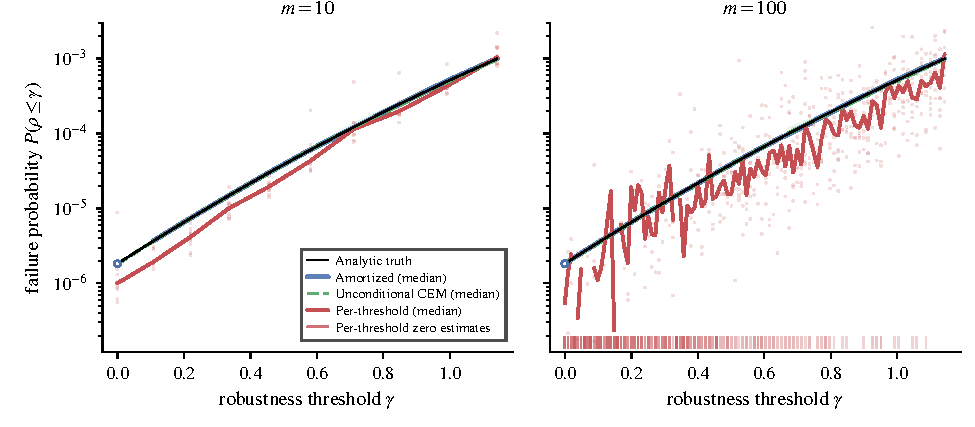
\includegraphics[width=0.9\linewidth]
        {figures/appendix/exp1_kscaling_curves.pdf}
    \caption{
    Representative failure-probability curves for the unimodal benchmark at \(m=10\) and \(m=100\) requested thresholds under the fixed total budget \(B=25{,}000\). The amortized and unconditional CEM medians closely track the analytic truth and therefore largely overlap visually, while the independently refitted per-threshold baseline becomes noisier and loses coverage at \(m=100\). Missing estimates are omitted rather than replaced by the \(1/B\) convention used for ILE.
    }
    \label{fig:exp1-additional-curves}
\end{figure}

\begin{table}[ht!]
    \centering
    \caption{
    Full-curve estimation as the number of requested thresholds increases under a fixed budget of $B=25{,}000$ robustness evaluations. ILE is computed over the full threshold grid, substituting $1/B$ only for missing, zero, or non-finite estimates. Coverage is the fraction of requested thresholds with a finite positive estimate. Values are medians over 10 seeds.
    }
    \label{tab:exp1-full-results}
    \begin{tabular}{@{}lrrr@{}}
        \toprule
        Method & $m$ & ILE & Coverage \\
        \midrule
        Amortized
            & 10  & 0.0146 & 100.0\% \\
            & 25  & 0.0151 & 100.0\% \\
            & 50  & 0.0152 & 100.0\% \\
            & 100 & 0.0149 & 100.0\% \\
        \midrule
        Unconditional CEM
            & 10  & 0.0177 & 100.0\% \\
            & 25  & 0.0184 & 100.0\% \\
            & 50  & 0.0190 & 100.0\% \\
            & 100 & 0.0190 & 100.0\% \\
        \midrule
        Per-threshold
            & 10  & 0.4628 & 100.0\% \\
            & 25  & 0.5385 & 100.0\% \\
            & 50  & 0.6768 & 96.0\% \\
            & 100 & 1.2000 & 55.5\% \\
        \bottomrule
    \end{tabular}
\end{table}

\begin{table}[ht!]
    \centering
    \caption{
    Sensitivity of integrated log-error to the value substituted for missing, zero, or non-finite estimates in the unimodal benchmark. Positive finite estimates are never clipped. The primary analysis uses the budget-resolution convention $1/B$, with $B=25{,}000$. Values are medians over 10 seeds.
    }
    \label{tab:exp1-floor-sensitivity}
    \begin{tabular}{@{}lrrrr@{}}
        \toprule
        Method & $m$ & $1/B$ & $10^{-6}$ & $10^{-8}$ \\
        \midrule
        Amortized
            & 10  & 0.0146 & 0.0146 & 0.0146 \\
            & 25  & 0.0151 & 0.0151 & 0.0151 \\
            & 50  & 0.0152 & 0.0152 & 0.0152 \\
            & 100 & 0.0149 & 0.0149 & 0.0149 \\
        \midrule
        Per-threshold
            & 10  & 0.4628 & 0.4628 & 0.4628 \\
            & 25  & 0.5385 & 0.5385 & 0.5385 \\
            & 50  & 0.6768 & 0.6502 & 0.7644 \\
            & 100 & 1.2000 & 1.6361 & 3.7036 \\
        \bottomrule
    \end{tabular}
\end{table}

% Section C.2
% --------------------------------------------------------------
\subsection{Multimodal Tail Benchmark Results}
\label{app:tail-benchmark-results}

\Cref{tab:tail-benchmark-results} gives the seed-level mode-discovery statistics underlying \cref{fig:conditioning-modes}. Both classifications are computed by the run itself; neither is assigned after the fact. A seed is classified as discovering all three lobes when at least one draw with $\rho(x)\leq 0$ falls in each of the one-sided $x_1$ tail and the two $x_2$ tails defined in \cref{app:tail-race}, counted over all $80{,}000$ pooled draws of the run. A seed is classified as amplified when the importance-weighted probability mass its estimate attributes to the two $x_2$ lobes exceeds $10\%$ of the true failure probability; because those lobes carry more than $98\%$ of that probability at every $c_2$, this is in practice a threshold on the accuracy of $\widehat P$, and it selects exactly the seeds with $\widehat P/P_{\mathrm{true}}>0.1$. A seed is classified as locked when no draw with $\rho(x)\leq 0$ falls in either $x_2$ tail. The two classifications are independent: neither implies the other, and 12 of the 18 amplified seeds discovered only two lobes. 

\begin{table}[ht!]
    \centering
    \caption{
    Mode discovery and probability estimation on the multimodal tail benchmark. ``All'' is the number of 10 seeds that discover all three failure lobes, and ``Ampl.'' is the number classified in the amplified regime. The final two columns report the median ratio between the estimated and true failure probability at $\gamma=0$. The unconditional aggregates at $c_2=16$, $18$, and $23$ each include one fallback-assisted run.
    }
    \label{tab:tail-benchmark-results}
    \begin{tabular}{@{}lrrrrrr@{}}
        \toprule
        & \multicolumn{2}{c}{Conditioned}
        & \multicolumn{2}{c}{Unconditional}
        & \multicolumn{2}{c}{$\widehat P/P$} \\
        $c_2$
        & All & Ampl.
        & All & Ampl.
        & Conditioned & Unconditional \\
        \midrule
        16 & 6/10 & 7/10 & 1/10 & 4/10 & 0.436  & 0.00837 \\
        18 & 3/10 & 3/10 & 0/10 & 1/10 & 0.00365 & 0.000887 \\
        20 & 5/10 & 2/10 & 0/10 & 0/10 & 0.00237 & 0.00182 \\
        23 & 1/10 & 1/10 & 0/10 & 0/10 & 0.0107  & 0.00848 \\
        \bottomrule
    \end{tabular}
\end{table}

The single-draw threshold is weak at the larger thresholds---under the nominal distribution alone, $80{,}000$ draws are expected to place $5.1$, $1.8$, $0.6$ and $0.1$ points beyond $|x_2|\geq\sqrt{c_2}$ for $c_2=16,18,20,23$. 

As a sensitivity analysis, and not as a redefinition of the reported metric, we recomputed the counts requiring at least five failing draws in each lobe rather than one: the conditioned counts become 4/10, 1/10, 0/10 and 0/10, and the unconditional counts become 0/10 at all four settings, for $c_2=16,18,20,23$ respectively. The values reported in \cref{tab:tail-benchmark-results} and \cref{fig:conditioning-modes} remain those of the single-draw criterion. Under the stricter criterion the conditioned method retains an advantage only at $c_2=16$ and $c_2=18$; in particular the 5/10 versus 0/10 difference at $c_2=20$ does not survive, so that difference is better read as transient contact with the $x_2$ lobes than as sustained representation of them.

The conditioned method improves mode discovery more consistently than it improves the final probability estimate. At every value of $c_2$, the conditioned method discovers all three lobes in more seeds than the unconditional baseline. It also enters the amplified regime more often overall ($13$ versus $5$ of $40$ seeds), although this gap is smaller than the discovery gap. Run-level regime labels depend on individual adaptive trajectories, so single-seed differences such as $1/10$ versus $0/10$ should not be interpreted. Both methods, however, retain substantial seed-to-seed variability at the target threshold. Because the conditioned method fits on the accumulated sample buffer while the unconditional baseline fits on elites from the current batch, part of the difference in mode retention may arise from this fitting-set difference rather than from conditioning alone. The results therefore support a narrower interpretation: the full conditioned method can improve access to and retention of rare-event modes, but it does not guarantee accurate estimation when the relevant tail modes remain poorly sampled.

\paragraph{Degenerate-fit sensitivity.}
One unconditional run in each of the $c_2=16$, $18$, and $23$ settings terminated because of a degenerate mixture fit and was completed using a targeted fallback verified not to alter known-good runs. These runs are retained as fallback-assisted. Restricting each affected aggregate to its nine clean runs changes the median $\widehat P/P$ from $0.00837$ to $0.00898$ at $c_2=16$, from $0.000887$ to $0.00114$ at $c_2=18$, and from $0.00848$ to $0.00849$ at $c_2=23$. None of the three fallback-assisted runs discovers all three lobes or reaches the amplified regime, so the clean-only all-three-lobe and amplification counts are $1/9$ and $4/9$ at $c_2=16$, $0/9$ and $1/9$ at $c_2=18$, and $0/9$ and $0/9$ at $c_2=23$, compared with $1/10$ and $4/10$, $0/10$ and $1/10$, and $0/10$ and $0/10$ in the reported aggregate. Retaining these runs therefore changes the unconditional rates only through the denominator, and the qualitative comparison is unchanged.

% Section C.3
% --------------------------------------------------------------
\subsection{High-Dimensional Driving Diagnostics}
\label{app:high-diagnostics}

The probability curves in \cref{fig:driving-curve} show that the amortized estimator produces finite positive estimates across the full driving evaluation grid. We report additional diagnostics here to distinguish adaptive-schedule reach, sampling of the target region, and estimator-weight concentration.

Across the 10 seeds, the smallest adaptive threshold reached by the amortized proposal has median $\gamma_{\min}=0.362$, with range $0.305\leq\gamma_{\min}\leq0.369$. The adaptive schedule reaches the target threshold $\gamma=0$ in no seed.

Schedule reach is distinct from estimator availability. All 10 seeds contain samples at or below $\gamma=0$, with 36 to 66 of the $25{,}000$ draws per seed taking the simulator's collision value $\rho=-0.01$. Because the pooled estimator reuses samples collected across the adaptive run, it produces a finite positive estimate at every evaluation threshold in all 10 seeds, despite the adaptive schedule itself never reaching the target.

The schedule stalls rather than descending gradually. In every seed, $\gamma^{(k)}$ falls from about $0.69$ to about $0.37$ within the first four batches and then shows little further progress. Estimator weights nevertheless become increasingly concentrated toward the rare tail. For the pooled balance-MIS estimator, the median effective-sample-size fraction over samples with $\rho\leq0.434$ is $0.0256$. In absolute terms, median effective sample size decreases from $201$ at $\gamma=0.434$ to $54.8$ near the terminal adaptive threshold and $5.8$ at $\gamma=0$. Despite this concentration, all 10 target-threshold estimates are finite and lie within a factor of $3.25$ of the reference probability.

Proposal-density evaluation adds substantial computation beyond simulator calls. For the original amortized runs, marginal-density evaluation and pooled re-indexing dominate wall-clock time. Because the corrected baseline reruns used different concurrency settings, we do not compare wall-clock times across methods. The reported evaluation budgets therefore measure simulator effort rather than total computational cost.

% ==============================================================
% D. REPRODUCIBILITY AND EXPERIMENTAL CONFIGURATION
% ==============================================================
\section{Reproducibility and Experimental Configuration}
\label{app:reproducibility}

All reported method and baseline runs use fixed random seeds and saved experiment configurations. The final repository release will include the source snapshot, configuration files, and experimental artifacts corresponding to the reported results. All experiments were run with Julia 1.12.6.

\begin{table}[ht!]
    \centering
    \small
    \caption{
    Configurations for the four reported experiments. \(B\) is the nominal robustness-evaluation budget; baseline counts may differ because oracle-tuning costs are charged. SGM denotes the structured Gaussian mixture used in the high-dimensional conditional proposal.
    }
    \label{tab:canonical-configurations}

    \begin{tabular}{@{}lrrrrll@{}}
        \toprule
        Experiment
        & $d$
        & $B$
        & Batch
        & Iter.
        & Proposal
        & Settings \\
        \midrule

        Amortization
        & 2
        & 25k
        & 1k
        & 25
        & Cond.\ EMGMM
        & $C=2,\ \alpha=0.2$ \\

        Radial shell
        & 2, 20
        & 25k, 50k
        & 1k
        & 25 / 50
        & Cond.\ EMGMM
        & $C=2,\ \alpha=0.2$ \\

        Multimodal tail
        & 2
        & 80k
        & 2k
        & 40
        & Cond.\ EMGMM
        & $C=3,\ \alpha=0.15$ \\

        Driving
        & 150
        & 25k
        & 1k
        & 25
        & Cond.\ SGM
        & $C=2,\ r=10,\ \alpha=0.2$ \\

        \bottomrule
    \end{tabular}
\end{table}

\Cref{tab:canonical-configurations} summarizes the primary experimental configurations. All experiments use the observed robustness value directly when fitting the joint model, corresponding to $\sigma=0$. Experiments 1--3 use no defensive nominal mixture ($\eta=0$), whereas Experiment 4 uses $\eta=0.1$. Thus, the diagnostics for Experiments 1--3 describe the adaptive proposal alone. All reported aggregates use 10 random seeds.

\paragraph{Amortization experiment.}
The unimodal experiment uses $X\sim\mathcal N(0,I_2)$ and $\rho(x)=3-\min(x_1,x_2)$. We evaluate
\[
    m\in\{10,25,50,100\}
\]
requested thresholds under a fixed total budget $B=25{,}000$. The amortized proposal uses a two-component conditional EMGMM, batch size $1{,}000$, 25 adaptive iterations, and adaptive quantile $\alpha=0.2$. Proposal-fitting weights are capped at 10; estimator weights are neither clipped nor self-normalized.

All four grids share the same endpoints and differ only in density. For each $m$, the reference probabilities are logarithmically spaced from $10^{-3}$ to $\Phi(-3)^2$, with thresholds obtained from
\[
    \gamma
    =
    3+\Phi^{-1}\!\left(\sqrt{p}\right).
\]

The conditional model appends robustness as an additional coordinate and fits a full-covariance Gaussian mixture to the resulting joint vector. A Gaussian jitter of standard deviation $10^{-4}$ is added to the robustness coordinate on every fit. If a component covariance has determinant below $10^{-3}$, the fitting routine adds $10^{-2}I$. All reported proposal checkpoints and estimates use these regularized covariances.

\paragraph{Per-threshold baseline.}
The per-threshold baseline fits an independent proposal at each requested threshold. For a grid of $m$ thresholds, each run receives budget $\lfloor B/m\rfloor$ and uses the same joint-model method as the amortized method while targeting only its assigned threshold. Its batch size is
\[
    N
    =
    \min\!\left(
        500,\;
        \max\!\left(50,\;\lfloor B/m\rfloor/10\right)
    \right),
\]
giving $N=250,100,50,$ and $50$ for $m=10,25,50,$ and $100$. Each threshold is estimated independently using the proposal-of-origin estimator in \cref{eq:batch-is}; no information is shared across thresholds.

\paragraph{Unconditional CEM baseline.}
The unconditional cross-entropy baseline uses the same problem, random seeds, threshold grids, and total budget $B=25{,}000$. Its proposal is an unconditional two-component Gaussian mixture with no robustness conditioning or defensive nominal mixture. The run uses 25 batches of $1{,}000$ evaluations: the first is sampled from the nominal distribution, and each later batch is sampled from the proposal fitted to the elite samples of the preceding batch, with fitting weights capped at 10. The elite set contains samples satisfying $\rho(x)\leq0$, augmented when necessary to the $n_{\mathrm{elite}}=200$ lowest-robustness samples. Unlike the amortized method, this baseline has no explicit threshold schedule $\gamma^{(k)}$.

For curve estimation, the 25 sampling distributions are pooled using the same balance-heuristic MIS estimator as for the amortized method. The unconditional Gaussian-mixture density is available in closed form, so no marginal quadrature is required. The same determinant-based covariance regularization described above is applied to fitted mixtures.

\paragraph{Radial-shell experiment.}
The shell experiment uses
\[
    d\in\{2,20\},
    \qquad
    B\in\{25{,}000,50{,}000\}.
\]
The amortized proposal uses a two-component conditional EMGMM with batch size $1{,}000$, adaptive quantile $\alpha=0.2$, and 25 or 50 adaptive iterations according to the budget. Proposal-fitting weights are capped at 10, and the conditional model uses the same joint-vector construction and numerical safeguards as in the amortization experiment.

For each dimension, the evaluation grid contains 16 thresholds with exact failure probabilities logarithmically spaced from $10^{-3}$ to $10^{-6}$. The amortized method is compared with oracle-tuned per-threshold importance sampling and oracle-tuned adaptive multilevel splitting (AMS). All robustness evaluations used during oracle selection are charged.

The per-threshold oracle evaluates batch sizes $N\in\{100,250,500\}$ independently at each threshold, with each threshold--candidate pair using a distinct deterministic random-number stream. Each candidate receives budget $\lfloor B/16\rfloor$ truncated to an integer number of batches. The candidate with smallest relative error against the closed-form probability is reported, and the cost of all candidates is charged.

The AMS oracle sweeps $p_0\in\{0.1,0.2,0.3\}$ and $n_{\mathrm{MCMC}}\in\{5,10\}$. The configuration with smallest median relative error across the grid is reported, and all six configurations are charged.

A run is counted as reaching the evaluation grid when it produces at least one finite positive estimate on the 16-threshold grid. The harness emits an estimate at threshold $\gamma$ only when $\gamma$ is at or above the smallest intermediate threshold reached by the adaptive schedule, so reaching a grid point requires substantially more than merely placing samples there. In all four $(d,B)$ cells, every seed produced samples at or below the loosest grid threshold, while the schedule reached that threshold in only $1$, $4$, $0$, and $0$ seeds. Zero coverage therefore reflects the adaptive schedule rather than absence of samples in the failure region. Unlike the driving experiment (\cref{app:high-diagnostics}), which reports the pooled estimate at every evaluation threshold, the shell experiment retains this emission rule. Its reported coverage therefore measures adaptive-schedule reach rather than estimator availability.

The per-threshold baseline can return zero estimates at individual thresholds; these are handled by the missing-estimate convention used for ILE. AMS values at the evaluation thresholds are obtained by linear interpolation in $(\gamma,\log\widehat P)$ between adaptive levels.

\paragraph{Multimodal tail experiment.}
The multimodal tail experiment uses
\[
    c_1=5.5,
    \qquad
    c_2\in\{16,18,20,23\},
\]
with target threshold $\gamma=0$. The conditioned proposal uses a three-component conditional EMGMM, while the unconditional baseline uses a three-component EMGMM without robustness conditioning. Both use batch size $2{,}000$, 40 adaptive iterations, adaptive quantile $\alpha=0.15$, total budget $80{,}000$, and fitting-weight cap 10.

The conditioned method fits its proposal on the accumulated sample buffer, whereas the unconditional baseline fits on elites from the current batch. Thus, the comparison differs in both robustness conditioning and fitting-set construction. The conditioned method otherwise uses the same joint-vector construction and numerical safeguards as in the amortization experiment.

One unconditional run in each of the $c_2=16$, $18$, and $23$ settings encountered a degenerate mixture fit and was completed using a targeted fallback verified not to alter known-good runs. These runs are retained as fallback-assisted, with the corresponding sensitivity analysis reported in \cref{app:tail-benchmark-results}.

\paragraph{Driving experiment.}
The driving experiment uses a $150$-dimensional disturbance input consisting of 30 decision steps and five channels per step. The decision interval is $0.2\,\mathrm{s}$ with four physics substeps, giving $\Delta t_{\mathrm{phys}}=0.05\,\mathrm{s}$, and the disturbance scale is $a_{\mathrm{scale}}=0.60$. The threshold grid is
\[
    \{0.434,\,0.38,\,0.32,\,0.26,\,0.20,\,0.14,\,0.08,\,0\}.
\]

The adaptive proposal uses a two-component conditional Gaussian model with low-rank-plus-diagonal covariance of rank 10 and a defensive nominal mixture with $\eta=0.1$. It uses batch size $1{,}000$, 25 adaptive iterations, and adaptive quantile $\alpha=0.2$. Because
\[
    q_\eta(x)
    =
    (1-\eta)q(x)+\eta p(x),
\]
the proposal-fitting weights satisfy
\[
    \frac{p(x)}{q_\eta(x)}
    \leq
    \frac{1}{\eta}
    =
    10.
\]
The reported curve uses pooled balance-heuristic MIS over the nominal distribution and the 24 fitted defensive-mixture proposals.

Covariance regularization for this model enforces a diagonal floor $D\geq10^{-4}$ at every inner M-step update. This floor is active in every seed, and some fitted components collapse toward the floor, producing highly concentrated densities and occasional importance-weight underflow. All reported proposal checkpoints and estimates use the floored covariances. A Gaussian jitter of standard deviation $10^{-4}$ is also added to the robustness coordinate on every fit; this is distinct from the smoothing parameter, which is $\sigma=0$.

The per-threshold baseline evaluates batch sizes $500$ and $1{,}000$ independently at each threshold, using $3{,}000$ evaluations per candidate. Each threshold--candidate pair uses a distinct deterministic random-number stream. The candidate closer to the reference probability is reported, and all $48{,}000$ evaluations are charged. Because the oracle selects the candidate with smaller relative error, it can prefer an exactly zero estimate to a positive overestimate. Of the 80 reported threshold--seed estimates, 24 are exactly zero, so per-threshold coverage reflects both sampling support and the oracle-selection rule.

AMS uses the same six-configuration oracle sweep as in the radial-shell experiment. Its random-walk mutation scale is
\[
    \sigma_{\mathrm{RWM}}
    =
    \frac{2.38}{\sqrt{d}},
\]
a standard dimension-scaled random-walk-Metropolis rule motivated by asymptotic optimal-scaling theory. We do not claim that this scale is optimal for the truncated AMS target. AMS terminates once the target level is reached, so its charged cost is data-dependent: across the 10 reported seeds, the total oracle cost ranges from $101{,}024$ to $125{,}936$ evaluations, with median $115{,}018$. Non-finite candidate outputs are excluded explicitly from oracle selection, and requested-grid probabilities are obtained from exact adaptive levels where available or by interpolation in $(\gamma,\log\widehat P)$ between valid levels.

The comparison reference contains $26$ million simulator rollouts using the same disturbance dimension, disturbance scale, physics discretization, and robustness definition as the experimental runs. Reference probabilities are evaluated at the exact requested thresholds using the histogram-edge convention described in \cref{app:idm}.

\paragraph{Marginal-density evaluation.}
Threshold-specific importance weights require
\[
    q_X^\gamma(x)
    =
    \int_{-\infty}^{\gamma}
    q_\psi(r\mid r\leq\gamma)
    q_\theta(x\mid r)\,dr.
\]
All joint-model experiments evaluate this integral using adaptive Gauss--Kronrod quadrature with relative tolerance
\[
    \mathrm{rtol}=10^{-3}.
\]
The mathematical domain is $(-\infty,\gamma]$. Numerically, the lower endpoint is truncated at the $10^{-12}$ quantile of the learned robustness marginal.

The canonical evaluator uses batched, vector-valued quadrature. Per-sample scaling converts the integrator's $L^\infty$ error criterion into an approximately relative error criterion for each $q_X^\gamma(x_i)$. These scales are obtained from a coarse 64-node pre-pass used only for normalization. Deterministic initial breakpoints are constructed from quantiles of the truncated robustness marginal and geometric offsets below $\gamma$, making the initialization independent of sample batching; subsequent node placement is adaptive.

The stored \texttt{quadrature\_nodes}=1000 field is an inactive legacy setting from a superseded fixed-grid evaluator and is not used by the canonical code path.

\paragraph{Artifacts.}
The accompanying repository release, \href{https://github.com/sisl/ARIS.jl}{\texttt{ARIS.jl}}, includes the fixed experiment configurations and stored outputs used to produce the reported tables, figures, and summary statistics. These artifacts permit recomputation of the reported estimates and diagnostics without rerunning the simulator.

\end{document}